\documentclass[draft,linenumbers]{agujournal2018}
%DIF LATEXDIFF DIFFERENCE FILE
%DIF DEL paper-submitted-1.tex   Tue Jul 16 17:41:03 2019
%DIF ADD paper.tex               Wed Jul 31 16:23:09 2019
\usepackage{apacite}
%DIF 3c3
%DIF < \usepackage{url} %this package should fix any errors with URLs in refs.
%DIF -------
\usepackage{url} % should fix any errors with URLs in refs. %DIF > 
%DIF -------
\usepackage{amsmath}
\usepackage{xcolor}
\usepackage[colorlinks]{hyperref}
\usepackage[colorinlistoftodos]{todonotes}
%DIF 8-22d8
%DIF < 
%DIF < %\usepackage{framebox}
%DIF < 
%DIF < %%%%%%%
%DIF < %\usepackage{trackchanges}
%DIF < % uncomment the line above to use the TrackChanges package to mark revisions if needed.
%DIF < % The trackchanges package adds five new LaTeX commands:
%DIF < %
%DIF < %  \note[editor]{The note}
%DIF < %  \annote[editor]{Text to annotate}{The note}
%DIF < %  \add[editor]{Text to add}
%DIF < %  \remove[editor]{Text to remove}
%DIF < %  \change[editor]{Text to remove}{Text to add}
%DIF < %
%DIF < % complete documentation is here: http://trackchanges.sourceforge.net/
%DIF -------

\draftfalse

\journalname{Space Weather}
%DIF PREAMBLE EXTENSION ADDED BY LATEXDIFF
%DIF UNDERLINE PREAMBLE %DIF PREAMBLE
\RequirePackage[normalem]{ulem} %DIF PREAMBLE
\RequirePackage{color}\definecolor{RED}{rgb}{1,0,0}\definecolor{BLUE}{rgb}{0,0,1} %DIF PREAMBLE
\providecommand{\DIFaddtex}[1]{{\protect\color{blue}\uwave{#1}}} %DIF PREAMBLE
\providecommand{\DIFdeltex}[1]{{\protect\color{red}\sout{#1}}}                      %DIF PREAMBLE
%DIF SAFE PREAMBLE %DIF PREAMBLE
\providecommand{\DIFaddbegin}{} %DIF PREAMBLE
\providecommand{\DIFaddend}{} %DIF PREAMBLE
\providecommand{\DIFdelbegin}{} %DIF PREAMBLE
\providecommand{\DIFdelend}{} %DIF PREAMBLE
\providecommand{\DIFmodbegin}{} %DIF PREAMBLE
\providecommand{\DIFmodend}{} %DIF PREAMBLE
%DIF FLOATSAFE PREAMBLE %DIF PREAMBLE
\providecommand{\DIFaddFL}[1]{\DIFadd{#1}} %DIF PREAMBLE
\providecommand{\DIFdelFL}[1]{\DIFdel{#1}} %DIF PREAMBLE
\providecommand{\DIFaddbeginFL}{} %DIF PREAMBLE
\providecommand{\DIFaddendFL}{} %DIF PREAMBLE
\providecommand{\DIFdelbeginFL}{} %DIF PREAMBLE
\providecommand{\DIFdelendFL}{} %DIF PREAMBLE
%DIF HYPERREF PREAMBLE %DIF PREAMBLE
\providecommand{\DIFadd}[1]{\texorpdfstring{\DIFaddtex{#1}}{#1}} %DIF PREAMBLE
\providecommand{\DIFdel}[1]{\texorpdfstring{\DIFdeltex{#1}}{}} %DIF PREAMBLE
%DIF END PREAMBLE EXTENSION ADDED BY LATEXDIFF

\begin{document}

%DIF <  Not working
%DIF <  \listoftodos
\DIFaddbegin \title{\DIFadd{A Test of the Frequency Independence Assumption of Power System Coefficients used in Geomagnetically Induced Current Estimates}}
\DIFaddend 

\DIFdelbegin %DIFDELCMD < \title{A Test of the Frequency Independence Assumption of Power System Parameters used in Geomagnetically Induced Current Estimates}
%DIFDELCMD < 

%DIFDELCMD < %%%
\DIFdelend \authors{R.S. Weigel\affil{1} and P.J. Cilliers\affil{2}}

%DIF < Weigel: http://orcid.org/0000-0002-9521-5228
%DIF < Cilliers: http://orcid.org/0000-0003-3175-5134
\DIFdelbegin %DIFDELCMD < 

%DIFDELCMD < %%%
\DIFdelend \affiliation{1}{Space Weather Lab, George Mason University}
\affiliation{2}{South African National Space Agency}

\affiliation{1}{4400 University Drive, Fairfax VA 22030}
\affiliation{2}{Hospital Street, Hermanus 7200}

\correspondingauthor{R.S. Weigel}{rweigel@gmu.edu}

\begin{keypoints}
\item Power system \DIFdelbegin \DIFdel{parameters }\DIFdelend \DIFaddbegin \DIFadd{coefficients }\DIFaddend derived from a time series of GIC and geoelectric field measurements are frequency dependent.
\item A GIC \DIFdelbegin \DIFdel{prediction }\DIFdelend model with frequency-dependent system \DIFdelbegin \DIFdel{parameters }\DIFdelend \DIFaddbegin \DIFadd{coefficients }\DIFaddend provides significantly better \DIFdelbegin \DIFdel{predictions }\DIFdelend \DIFaddbegin \DIFadd{estimates of GIC }\DIFaddend than a frequency independent model.
\item \DIFdelbegin \DIFdel{A model derived using GIC and geomagnetic field data provides better predictions than a GIC and geoelectric field-based model}\DIFdelend \DIFaddbegin \DIFadd{Data-derived power system coefficients may differ significantly with those computed using power system configuration information}\DIFaddend .
\end{keypoints}

\begin{abstract}
  A common assumption used when estimating geomagnetically induced currents (GICs) in a power system given a time series of nearby direct measurements or indirect estimates of the horizontal geoelectric field components $E_x(t)$ and $E_y(t)$ on Earth's surface is that the system is resistive. That is, the approximation $GIC(t)$  $=$ $a_oE_x(t) + b_oE_y(t)$ (Model 1) is used, where $a_o$ and $b_o$ are frequency-independent \DIFdelbegin \DIFdel{network parameters}\DIFdelend \DIFaddbegin \DIFadd{power system coefficients}\DIFaddend .  A first test of this assumption is made using GIC measurements \DIFdelbegin \DIFdel{made }\DIFdelend in a 187 kV transformer connected to a $\sim$100~km power line in Memanbetsu, Japan and geoelectric field measurements made at the Memanbetsu Magnetic Observatory $\sim$9~km away. A second model (Model 2) is obtained using a frequency domain generalization of Model 1: $GIC(\omega)$ $=$ $a(\omega)E_x(\omega) + b(\omega)E_y(\omega)$. The \DIFdelbegin \DIFdel{network parameters }\DIFdelend \DIFaddbegin \DIFadd{coefficients }\DIFaddend $a(\omega)$ and $b(\omega)$ are computed from data and are shown to be frequency dependent and this model provides significantly better estimates of the measured GIC than Model\DIFaddbegin \DIFadd{~}\DIFaddend 1. \DIFdelbegin \DIFdel{A third model, which uses the electric field estimated by convolving a magnetotelluric transfer function with the geomagnetic field, provides significantly better estimates over Model~2. }\DIFdelend Based on results using a simulated geoelectric field, it is suggested that the measurement-derived frequency dependence of the system \DIFdelbegin \DIFdel{parameters }\DIFdelend \DIFaddbegin \DIFadd{coefficients }\DIFaddend may be explained by spatial variations in the spectrum of the geoelectric field along the line in which GIC is measured rather than by an actual frequency dependence of the system \DIFdelbegin \DIFdel{parameters. }%DIFDELCMD < 

%DIFDELCMD < %%%
%DIF < Network parameters $a(\omega)$ and $b(\omega)$ computed from data in Model 2, $GIC(\omega)$ $=$ $a(\omega)E_x(\omega) + b(\omega)E_y(\omega)$, are shown to be frequency dependent and this model provides a significantly better estimates of the measured GIC over Model~1. 
%DIFDELCMD < 

%DIFDELCMD < %%%
%DIF < It is suggested that the measurement-derived frequency dependence of the system parameters is explained by spatial variations in the spectrum of the geoelectric field along the line in which GIC is measured rather than by an actual frequency dependence of the system parameters.
%DIFDELCMD < 

%DIFDELCMD < %%%
\DIFdelend \DIFaddbegin \DIFadd{components. It is also shown that further improvements over Model~2 can be made using models with the geomagnetic field as an input.
}\DIFaddend \end{abstract}

\section{Introduction}

Geomagnetically induced currents (GICs) are electric currents in conducting systems that are due to electric fields near the Earth's surface. Time-varying electric and magnetic fields at Earth's surface are driven by time variations in ionospheric currents on time scales \DIFdelbegin \DIFdel{on the order of }\DIFdelend \DIFaddbegin \DIFadd{of seconds to }\DIFaddend hours \citep{Ohtani2000} and the movement of Earth's surface relative to slow-varying current systems in Earth's ionosphere that are near stationary relative to the Sun \citep{Stening2013}. Of particular interest are currents induced in electric power systems because they can lead to system degradation, disruption, and failure \citep{Albertson1993,NERC2012,Gaunt2014}. Accurate estimation of GIC magnitudes is important for power system design, retrospective analysis, and mitigation of the impacts of space weather on power systems \citep{Molinski2002,Thomson2010,NERC2012,Gaunt2014}.

A common assumption made in estimates of GIC in an electric power system using either a measured or estimated time series of the horizontal geoelectric field at Earth's surface, $\mathbf{E}(t)$, is that the power system is resistive or quasi-DC in the sense that the relationship $GIC(t) = a_oE_x(t) + b_oE_y(t)$ holds \citep{Albertson1981,Lehtinen1985}. In this case, estimates of the coefficients $a_o$ and $b_o$ can be easily made from the data using linear regression when contemporaneous measurements of $GIC(t)$ and $\mathbf{E}(t)$ are available, or by using information about the connectivity of the power lines and values of the conductor and transformer resistances using DC circuit methods \citep[e.g.,][]{Boteler2014a,Boteler2014b,Boteler2017}. This quasi-DC assumption has been used or stated in many GIC-related works, for example, \DIFdelbegin %DIFDELCMD < \citet{Pulkkinen2007,Wik2008,Pulkkinen2010,Ngwira2011,Horton2012,Viljanen2012,Overbye2012,Marshall2013,Liu2014,Zheng2014,Watari2015,Bonner2017}%%%
\DIFdelend \DIFaddbegin \citet{Pulkkinen2007,Wik2008,Pulkkinen2010,Ngwira2011,Horton2012,Viljanen2012,Overbye2012,Marshall2013,Liu2014,Zheng2014,Watari2015}\DIFaddend .

%DIF < \cite{Oyedokun2013a} developed a method to account for the finite inductive response time of transformers by taking the GIC predicted based on the quasi-DC assumption and then applying a piecewise-linear L/R filter derived from bench-scale transformer measurements, with a time constant dependent on load, to obtain an alternative estimate of GIC. 
\DIFdelbegin %DIFDELCMD < 

%DIFDELCMD < %%%
%DIF < \todo[inline]{What can I conclude from \cite{Oyedokun2013a}? Mostly the thesis documents visual differences in time series traces with and without accounting for transformers.} 
%DIFDELCMD < 

%DIFDELCMD < %%%
\DIFdelend In this work, we use a unique dataset in which time series measurements of $\mathbf{E}$ and the surface horizontal geomagnetic field, $\mathbf{B}$, were made near a site where GIC was being measured in an electric power system.  We first estimate the system \DIFdelbegin \DIFdel{parameters }\DIFdelend \DIFaddbegin \DIFadd{coefficients }\DIFaddend $a_o$ and $b_o$ from data using conventional methods, in which they are modeled as frequency independent. Then, we use a model in which the system \DIFdelbegin \DIFdel{parameters }\DIFdelend \DIFaddbegin \DIFadd{coefficients }\DIFaddend are allowed to be frequency dependent, compute the frequency dependence, and compare this model's ability to represent GIC with the traditional frequency-independent model. \DIFaddbegin \DIFadd{Two additional models are considered that require only the geomagnetic field as an input and they are shown to be significantly better at estimating GIC than the models that use only the geoelectric field as an input.
}\DIFaddend 

\section{Data}

The 1-second-cadence GIC data used span a total of 35 days across 10 intervals that start and end at midnight Japan Standard Time (JST) and are listed in Table~\ref{intervals}. These data have been presented previously in \citet{Watari2009} and \cite{Watari2015}. These time intervals are those for which GIC data was made available with the exception of three days for which there were obvious problems with either the electric field or GIC measurements. The GIC dataset includes 1~s raw data and 1~Hz low-pass-filtered raw measurements \DIFdelbegin \DIFdel{. The results presented here }\DIFdelend \DIFaddbegin \DIFadd{and the results presented }\DIFaddend are for the 1~Hz low-pass-filtered GIC measurements\DIFaddbegin \DIFadd{.
}\DIFaddend 

\DIFdelbegin %DIFDELCMD < \begin{table}
%DIFDELCMD < %%%
%DIFDELCMD < \caption{%
{%DIFAUXCMD
\DIFdelFL{Date intervals used for analysis}}
%DIFAUXCMD
%DIFDELCMD < \centering
%DIFDELCMD < \begin{tabular}{l l}
%DIFDELCMD < \hline
%DIFDELCMD < %%%
\DIFdelFL{Start Date }%DIFDELCMD < & %%%
\DIFdelFL{End Date}%DIFDELCMD < \\
%DIFDELCMD < \hline
%DIFDELCMD < %%%
\DIFdelFL{2006-04-03 }%DIFDELCMD < & %%%
\DIFdelFL{2006-04-10}%DIFDELCMD < \\
%DIFDELCMD < %%%
\DIFdelFL{2006-07-25 }%DIFDELCMD < & %%%
\DIFdelFL{2006-07-29}%DIFDELCMD < \\
%DIFDELCMD < %%%
\DIFdelFL{2006-08-05 }%DIFDELCMD < & %%%
\DIFdelFL{2006-08-08}%DIFDELCMD < \\
%DIFDELCMD < %%%
\DIFdelFL{2006-08-19 }%DIFDELCMD < & %%%
\DIFdelFL{2006-08-21}%DIFDELCMD < \\
%DIFDELCMD < %%%
\DIFdelFL{2006-11-07 }%DIFDELCMD < & %%%
\DIFdelFL{2006-11-12}%DIFDELCMD < \\
%DIFDELCMD < %%%
\DIFdelFL{2006-11-28 }%DIFDELCMD < & %%%
\DIFdelFL{2006-11-29}%DIFDELCMD < \\
%DIFDELCMD < %%%
\DIFdelFL{2006-12-01 }%DIFDELCMD < & %%%
\DIFdelFL{2006-12-14}%DIFDELCMD < \\
%DIFDELCMD < %%%
\DIFdelFL{2006-12-15 }%DIFDELCMD < & %%%
\DIFdelFL{2006-12-15}%DIFDELCMD < \\
%DIFDELCMD < %%%
\DIFdelFL{2007-11-18 }%DIFDELCMD < & %%%
\DIFdelFL{2007-11-20}%DIFDELCMD < \\
%DIFDELCMD < %%%
\DIFdelFL{2007-11-22 }%DIFDELCMD < & %%%
\DIFdelFL{2007-11-22}%DIFDELCMD < \\
%DIFDELCMD < \hline
%DIFDELCMD < \end{tabular}
%DIFDELCMD < \label{intervals}
%DIFDELCMD < \end{table}
%DIFDELCMD < %%%
\DIFdelend \DIFaddbegin \DIFadd{GIC was measured in a grounded neutral point of a Y-connected three-phase transformer connected to the 187 kV bus at the Memanbetsu substation of the Hokkaido Power Co. The 187 kV line extends from the Ashro to Memanbetsu substation, which are both grounded. Memanbetsu is an end point of the line.
}\DIFaddend 

One-second-cadence electric and magnetic field measurements from \DIFdelbegin \DIFdel{Memambetsu Magnetic Observatory }\DIFdelend \DIFaddbegin \DIFadd{Memanbetsu Magnetic Observatory (geodetic latitude: 43.910$^{\circ}$ N, geodetic longitude: 144.189$^{\circ}$ E) }\DIFaddend were obtained from the Japan Meteorological Agency data portal. \DIFaddbegin \DIFadd{The location of the observatory and substation are shown in Figure~\ref{map}.
}\DIFaddend 

Data for the time span of 2006-08-04T15:\DIFdelbegin \DIFdel{00 }\DIFdelend \DIFaddbegin \DIFadd{00Z }\DIFaddend through 2006-08-08T15:\DIFdelbegin \DIFdel{00 }\DIFdelend \DIFaddbegin \DIFadd{00Z }\DIFaddend are shown Figure~\ref{sample}. The GIC data were provided as 1-day files that start at midnight JST and the times shown in Figure~\ref{sample} are Universal Time.

Spikes in the electric field measurements were assumed to be unphysical when the absolute value of a component $i$ of the electric field changed by more than 1~mV/km at time $t$, and the values $E_i(t-2)$ through $E_i(t+4)$ were replaced using linear interpolation of the values at $E_i(t-3)$ and $E_i(t + 5)$. In the sample shown in Figure~\ref{sample}, 21 spikes were identified in $E_x$ and zero in $E_y$. For \DIFdelbegin \DIFdel{all of }\DIFdelend the time intervals considered, the fraction of interpolated electric field values ranged from 0--0.1\%.

The only modification made to the magnetic field measurements was the replacement of 36 data points on 2006-08-06 with linearly interpolated values. The 36 \DIFdelbegin \DIFdel{values }\DIFdelend \DIFaddbegin \DIFadd{data points }\DIFaddend for $B_x$ and $B_y$ \DIFdelbegin \DIFdel{were the same and }\DIFdelend \DIFaddbegin \DIFadd{have the same value and are }\DIFaddend much larger than the surrounding values.

The GIC data contains non-physical spikes that are followed by 40-80~s of anomalous values that appear as an exponential decay back to pre-spike values. These spikes were removed by identifying times $t$ when the change in the 1~s absolute value of $GIC(t)$ was greater than $0.05$~Amps and then values in a window $GIC(t-2)$ through $GIC(t+100)$ were replaced using a linear interpolation of the values at $GIC(t-3)$ and $GIC(t + 101)$. In the example interval shown in Figure~\ref{sample}, 493 spikes were removed. For \DIFdelbegin \DIFdel{all of }\DIFdelend the time intervals considered, the fraction of interpolated GIC values ranged from 1--4\%.

\section{Models and Methods}
\DIFaddbegin \label{section:Models_and_Methods}
\DIFaddend 

To determine the coefficients $a_o$ and $b_o$ in the frequency independent model, Model~1,

\begin{linenomath*}
  \begin{equation}
    G_o(t) = a_oE_x(t) + b_oE_y(t)
    \label{model1}
  \end{equation}
\end{linenomath*}

\noindent
the matrix equation $\underline{\mathbf{GIC}} = \underline{\mathbf{E}}\cdot\mathbf{p}$ is solved in a least squares sense, where $\underline{\mathbf{GIC}}$ is a zero mean 86400x1 matrix with rows of $GIC(t)$; $\mathbf{p} = [a_o,b_o]^T$, and $\underline{\mathbf{E}}$ is a 86400x2 matrix with rows of $[E_x(t), E_y(t)]$ with zero mean columns. The values of $a_o$ and $b_o$ determined in this way correspond to those that minimize the sum-of-squares of $GIC(t)-G_o(t)$ over a 1-day interval. \citep[][provided the mathematically equivalent closed-form equations for solving the matrix equation.]{Pulkkinen2007} The notation $\overline{a}_o$ and $\overline{b}_o$ will be used for the average of the $a_o$ and $b_o$ values computed using the 35 1-day window segments of available data.

In Model\DIFaddbegin \DIFadd{~}\DIFaddend 2, the system \DIFdelbegin \DIFdel{parameters }\DIFdelend \DIFaddbegin \DIFadd{coefficients }\DIFaddend $a(\omega)$ and $b(\omega)$ are frequency dependent according to \DIFaddbegin \DIFadd{(frequency-dependent variables are indicated by explicitly listing their dependence on $\omega$)
}\DIFaddend 

\begin{linenomath*}
  \begin{equation}
    G_E(\omega) = a(\omega)E_x(\omega) + b(\omega)E_y(\omega)
    \label{model2}
  \end{equation}
\end{linenomath*}
\noindent
and \DIFdelbegin \DIFdel{are computed using contemporaneous measurements }\DIFdelend \DIFaddbegin \DIFadd{were estimated using the Fourier transforms }\DIFaddend of  $GIC(t)$ and $\mathbf{E}(t)$\DIFdelbegin \DIFdel{. The method of parameter estimation and generating predictions for Models 2-4 }\DIFdelend \DIFaddbegin \DIFadd{; the method of coefficient estimation and the generation of time-domain GIC estimates for this and the following models }\DIFaddend are given at the end of this section\DIFdelbegin \DIFdel{and fourier transformed variables are indicated by explicitly listing their dependence on $\omega$. }\DIFdelend \DIFaddbegin \DIFadd{.
}\DIFaddend 

\DIFaddbegin \DIFadd{Motivated by the results described in the following section, in which Model~2 provides a significantly better representation of GIC than Model~1, we have also considered two additional models that can be used to estimate GIC. In these two models, a direct measurement of the geoelectric field is not used; instead, the driver is the geomagnetic field, which is much more frequently measured, and as a result, these models may be of practical interest.
}

\DIFaddend In Model~3, the \DIFdelbegin \DIFdel{parameters }\DIFdelend \DIFaddbegin \DIFadd{coefficients }\DIFaddend $a(\omega)$ and $b(\omega)$ from Model~2 are used, but with an electric field $\mathbf{E}'$ computed using the measured magnetic field, $\mathbf{B}$, and a transfer function $\boldsymbol{Z}$: $\mathbf{E}'(\omega) \equiv \boldsymbol{Z}(\omega)\mathbf{B}(\omega)$ and

\setcounter{equation}{2}
\begin{linenomath*}
  \begin{equation}
    G_{E'}(\omega) = a(\omega)E'_x(\omega) + b(\omega)E'_y(\omega)
    \label{model3}
  \end{equation}
\end{linenomath*}

\noindent
where, explicitly, the electric field components are $E'_x$ = $Z_{xx}B_x + Z_{xy}B_y$ and $E'_y = Z_{yx}B_x + Z_{yy}B_y$.
That is, instead of using the measured electric field directly as in Model\DIFaddbegin \DIFadd{~}\DIFaddend 2, a magnetotelluric transfer function that relates $\mathbf{E}$ to $\mathbf{B}$ is used to provide an estimate of the electric field based on the magnetic field.

%DIF < Substitution gives
\DIFdelbegin %DIFDELCMD < 

%DIFDELCMD < %%%
%DIF < \begin{linenomath*}
%DIF < \begin{equation*}
%DIF < G_{E'}(\omega) = %\big[a(\omega)Z_{xx}(\omega) + b(\omega)Z_{yx}(\omega) \big] B_x(\omega) + \big[ a(\omega)Z_{xy}(\omega) + b(\omega)Z_{yy}(\omega) \big] B_y(\omega)\,.
%DIF < \end{equation*}
%DIF < \end{linenomath*}
%DIFDELCMD < 

%DIFDELCMD < %%%
\DIFdelend The fourth model is

\begin{linenomath*}
  \begin{equation}
    G_B(\omega) = z_x(\omega)B_x(\omega) + z_y(\omega)B_y(\omega)\,.
    \label{model4}
  \end{equation}
\end{linenomath*}

\noindent
In this model, the transfer function components $z_x$ and $z_y$ are determined directly from measurements of $GIC(t)$ and $\mathbf{B}(t)$ and no electric field measurements are used; this model is expected to produce \DIFdelbegin \DIFdel{predictions }\DIFdelend \DIFaddbegin \DIFadd{estimates }\DIFaddend of GIC that are similar to that obtained from Model\DIFaddbegin \DIFadd{~}\DIFaddend 3 because they both use the same input \DIFdelbegin \DIFdel{variable}\DIFdelend \DIFaddbegin \DIFadd{measurements}\DIFaddend .

Estimates of $a(\omega)$ and $b(\omega)$ are made at evaluation frequencies, $\omega_e \equiv 2\pi f_e$, by performing a ordinary least squares regression (OLS) using Equation~\ref{model2} and a set $G_E(\omega)$ and $\mathbf{E}(\omega)$ \DIFdelbegin \DIFdel{values near }\DIFdelend \DIFaddbegin \DIFadd{in a band of frequencies around }\DIFaddend $f_e$ from the DFT (discrete \DIFdelbegin \DIFdel{fourier }\DIFdelend \DIFaddbegin \DIFadd{Fourier }\DIFaddend transform) of 24 hours of 1-s cadence data. Following the suggestion of \cite{Simpson2005}, the 28 values of $f_e$ start at $0.25$ Hz and decrease by a factor of $\sqrt{2}$ and end at $1/43200$~Hz; if a $f_e$ value computed in this way is not an integer multiple of $1/86400$, the nearest smaller integer multiple is used. The \DIFaddbegin \DIFadd{periods associated with the evaluation frequencies are listed in Table~\ref{evaluationperiods}. The }\DIFaddend regression for each $f_e$ uses all DFT frequencies with values in a \DIFdelbegin \DIFdel{window }\DIFdelend \DIFaddbegin \DIFadd{band }\DIFaddend with a width of twice the separation from the next lower value of $f_e$ and the given $f_e$ with the exceptions that the lowest \DIFdelbegin \DIFdel{evaluation window }\DIFdelend \DIFaddbegin \DIFadd{band }\DIFaddend has a lower bound of $1/86400$~Hz and highest \DIFdelbegin \DIFdel{evaluation window }\DIFdelend \DIFaddbegin \DIFadd{band }\DIFaddend has an upper bound of \DIFdelbegin \DIFdel{$0.5$}\DIFdelend \DIFaddbegin \DIFadd{$0.375$}\DIFaddend ~Hz.

The same approach is used for solving for $z_x$ and $z_y$ in Equation~\ref{model4}. For the transfer function $\boldsymbol{Z}$ in $\mathbf{E}(\omega) = \boldsymbol{Z}(\omega)\mathbf{B}(\omega)$ used in Model~3, the $xx$ and $xy$ components of $\boldsymbol{Z}$ are solved for using

\begin{linenomath*}
  \begin{equation*}
    E_x(\omega) = Z_{xx}(\omega)B_x(\omega) + Z_{xy}(\omega)B_{y}(\omega)
  \end{equation*}
\end{linenomath*}

\noindent
and the $yx$ and $yy$ components are solved for using

\begin{linenomath*}
  \begin{equation*}
    E_y(\omega) = Z_{yx}(\omega)B_x(\omega) + Z_{yy}(\omega)B_y(\omega)
  \end{equation*}
\end{linenomath*}

Transfer \DIFdelbegin \DIFdel{function parameters }\DIFdelend \DIFaddbegin \DIFadd{functions }\DIFaddend were computed for each of the \DIFaddbegin \DIFadd{1-day }\DIFaddend segments. The average transfer function magnitude and phase at a given evaluation frequency was obtained by averaging the segment values at that evaluation frequency.

To interpolate the frequency-domain transfer function \DIFdelbegin \DIFdel{parameters }\DIFdelend \DIFaddbegin \DIFadd{components }\DIFaddend estimated at the evaluation frequencies, their real and imaginary components \DIFdelbegin \DIFdel{are }\DIFdelend \DIFaddbegin \DIFadd{were }\DIFaddend linearly interpolated individually onto the original DFT frequency grid (with a spacing of $1/86400$~Hz), and then the inverse DFT \DIFdelbegin \DIFdel{is }\DIFdelend \DIFaddbegin \DIFadd{was }\DIFaddend computed. The interpolated transfer function \DIFdelbegin \DIFdel{parameters }\DIFdelend \DIFaddbegin \DIFadd{coefficients }\DIFaddend were set to zero at frequencies higher than \DIFdelbegin \DIFdel{$0.25$}\DIFdelend \DIFaddbegin \DIFadd{$0.375$}\DIFaddend ~Hz and the transfer function estimate at $f=0$ was set to zero before interpolation.

\DIFdelbegin \DIFdel{Prediction }\DIFdelend \DIFaddbegin \DIFadd{GIC }\DIFaddend time series were calculated by \DIFdelbegin \DIFdel{convolution }\DIFdelend \DIFaddbegin \DIFadd{multiplication }\DIFaddend of the interpolated transfer function \DIFdelbegin \DIFdel{parameters }\DIFdelend \DIFaddbegin \DIFadd{coefficients }\DIFaddend with the DFT of the 24-hr long and 1~s cadence model inputs and computing the inverse DFT (e.g, for Model~2, $G_E(f)=a^I(f)E_x(f)+b^I(f)E_y(f)$ was calculated, where the superscript $I$ indicates the interpolated value, and then the inverse DFT of $G_E(f)$ was calculated to give the \DIFdelbegin \DIFdel{prediction }\DIFdelend \DIFaddbegin \DIFadd{estimate of }\DIFaddend $G_E(t)$ on a 1~s time grid).

Several modifications to this basic procedure were considered. Robust regression \citep{Egbert1986} with a Huber weighting constant of $1.345$ and an upper limit of 50 iterations and bi-square weighting with a constant of $4.685$ (both constants provide 95\% efficiency for \DIFdelbegin \DIFdel{normally distributed }\DIFdelend \DIFaddbegin \DIFadd{gaussian-distributed }\DIFaddend errors), both with no hard-cutoff step; time domain pre-whitening and tapering; and weighting the frequencies around each evaluation frequency using Parzen window weights. When using these additional steps individually, we find that the conclusions made regarding the differences each model's prediction ability do not change because the differences in each model's prediction performance are within the calculated uncertainty of the used method. Transfer function \DIFdelbegin \DIFdel{parameter values }\DIFdelend \DIFaddbegin \DIFadd{coefficients }\DIFaddend found using these modifications are generally within the error bars of those for the used procedure when the signal to noise ratio is above $\sim$3 (corresponding to periods \DIFdelbegin \DIFdel{higher than $\sim30$}\DIFdelend \DIFaddbegin \DIFadd{longer than $\sim$30}\DIFaddend ~s; At periods \DIFdelbegin \DIFdel{below }\DIFdelend \DIFaddbegin \DIFadd{shorter than }\DIFaddend $\sim$30~s, the electric field measurements are significantly influenced by the instrument response characteristics~\citep{Fujii2015}, aliasing, and the computed values are also expected to be significantly biased due to \DIFdelbegin \DIFdel{low signal to noise }\DIFdelend \DIFaddbegin \DIFadd{a low signal-to-noise }\DIFaddend ratio.)

\section{\DIFdelbegin \DIFdel{Results}\DIFdelend \DIFaddbegin \DIFadd{Model Evaluation}\DIFaddend }
\DIFaddbegin \label{section:Model_Evaluation}
\DIFaddend 

Out-of-sample \DIFdelbegin \DIFdel{prediction }\DIFdelend \DIFaddbegin \DIFadd{estimation quality }\DIFaddend metrics for each model on day $D$ were determined by computing the average model \DIFdelbegin \DIFdel{parameters }\DIFdelend \DIFaddbegin \DIFadd{coefficients }\DIFaddend using the remaining 34 days of data and then using these averaged \DIFdelbegin \DIFdel{parameters to generate a prediction }\DIFdelend \DIFaddbegin \DIFadd{coefficients to generate GIC }\DIFaddend time series and associated metrics on day $D$. This process was repeated to create a set of 35 out-of-sample prediction metrics for each model. In calculating the metrics, the first and last 10 minutes of the day were excluded to reduce the influence of transients that exist in the \DIFdelbegin \DIFdel{prediction }\DIFdelend \DIFaddbegin \DIFadd{estimate }\DIFaddend at the start of the interval for the amount of time that the causal part of the \DIFdelbegin \DIFdel{impulse response }\DIFdelend \DIFaddbegin \DIFadd{transfer function impulse responses (computed by Fourier inversion of the interpolated transfer function components) }\DIFaddend is non-zero and at the end for the amount of time that the acausal part of the impulse \DIFdelbegin \DIFdel{response is }\DIFdelend \DIFaddbegin \DIFadd{responses are }\DIFaddend non-zero.

The performance of each model in \DIFdelbegin \DIFdel{predicting }\DIFdelend \DIFaddbegin \DIFadd{estimating }\DIFaddend GIC was assessed using three metrics: the prediction efficiency, PE, the mean-squared-error (MSE) ratio, and the signal-to-noise ratio \DIFaddbegin \DIFadd{(SN)}\DIFaddend .

The \DIFdelbegin \DIFdel{prediction }\DIFdelend \DIFaddbegin \DIFadd{mean-squared-error for model $m$ on day $D$ is
}\begin{equation*}
  \DIFadd{\mbox{MSE}_m = \frac{1}{N}\sum_{t=t_o}^{t_f} \big(GIC(t)-GIC_m(t)\big)^2 \,,
}\end{equation*}
\noindent
\DIFadd{where $GIC_m(t)$ is the model prediction of model $m$ at time step $t$, $t_o=600$, and $t_f=85800$, so that sum is over one day of one-second-cadence measurements excluding the first and last 10~minutes. The MSE ratio for model $m$ is MSE$_1$/MSE$_m$.
}

\DIFadd{The prediction }\DIFaddend efficiency, PE, is the ``Case I'' skill score described by \cite{Murphy1988} and is \DIFdelbegin \DIFdel{defined as PE = 1 - variance(Prediction Error)/variance(Predicted); it }\DIFdelend \DIFaddbegin \DIFadd{calculated for day $D$ using
}\begin{equation*}
  \DIFadd{\mbox{PE}_m = 1 - \frac{\sum_{t=t_o}^{t_f} \big(GIC(t)-GIC_m(t)\big)^2}{\sum_{t=t_o}^{t_f} \big(GIC(t)-\overline{GIC(t)}\big)^2}\,,
}\end{equation*}
\noindent
\DIFadd{where $\overline{GIC(t)}$ is an average over the same time interval used in the summations. The PE }\DIFaddend is a measure of the skill of the model relative to the variance in the data that are predicted and it represents the fraction of the variance in the data that \DIFaddbegin \DIFadd{is }\DIFaddend predicted by the model.

The average PE and \DIFaddbegin \DIFadd{the }\DIFaddend MSE ratios were computed by averaging the out-of-sample \DIFdelbegin \DIFdel{PE }\DIFdelend \DIFaddbegin \DIFadd{PEs }\DIFaddend and MSE ratios\DIFdelbegin \DIFdel{; the average signal-to-noise ratio at a given frequency is the average of the out-of-sample signal-to-noise ratios at that frequency}\DIFdelend . The 95\% confidence interval, CI, on the PE and MSE ratio was calculated using \DIFdelbegin \DIFdel{1000 bootstrap }\DIFdelend \DIFaddbegin \DIFadd{the bootstrap method }\citep{Zoubir1998}\DIFadd{: 1000 }\DIFaddend samples of the out-of-sample prediction metrics \DIFaddbegin \DIFadd{were used to compute the CIs}\DIFaddend . (The typical difference between the limits when the confidence intervals were computed assuming the values were Gaussian-distributed was $\sim$2\%.)
\DIFdelbegin \DIFdel{The spectra for the signal and prediction error for each of the segments at a given evaluation frequency}\DIFdelend \DIFaddbegin 

\DIFadd{The signal-to-noise ratio on day $D$ at a given evaluation frequency is the ratio of of the smoothed power spectrum value of $GIC(\omega_e)$ to the smoothed power spectrum value of the prediction error at that evaluation frequency. A smoothed spectrum }\DIFaddend was obtained by averaging the raw \DIFdelbegin \DIFdel{spectra using }\DIFdelend \DIFaddbegin \DIFadd{spectrum in }\DIFaddend the same frequency \DIFdelbegin \DIFdel{windows }\DIFdelend \DIFaddbegin \DIFadd{bands }\DIFaddend used for the regression \DIFdelbegin \DIFdel{. 
}\DIFdelend \DIFaddbegin \DIFadd{described in Section~\ref{section:Models_and_Methods}. The average signal-to-noise ratio at a given evaluation frequency is the average of the 35 out-of-sample signal-to-noise ratios at that frequency.
}\DIFaddend 

\DIFaddbegin \section{\DIFadd{Results}}
\label{results}

\DIFadd{The PE and MSE ratios are shown in Table~\ref{results}. Figure~\ref{predictions} shows the predictions for each model in a 1-day interval selected because the value of the prediction efficiency for each model was in the same order as that shown in Table~\ref{results}, i.e., Model~1 has the lowest PE and Model~4 has the highest. Note that the large errors visible at the start and end of the time intervals are due to the transients discussed in Section~\ref{section:Model_Evaluation} and the first and last 10~minutes of each interval were omitted from metrics calculations.
}

\DIFaddend \begin{table}
  \caption{Out-of-sample model performance metrics for \DIFdelbeginFL \DIFdelFL{models $m=1-4$}\DIFdelendFL \DIFaddbeginFL \DIFaddFL{Model $m$}\DIFaddendFL . MSE\DIFdelbeginFL \DIFdelFL{$_m$}\DIFdelendFL \DIFaddbeginFL \DIFaddFL{$_1$}\DIFaddendFL /MSE\DIFdelbeginFL \DIFdelFL{$_1$ }\DIFdelendFL \DIFaddbeginFL \DIFaddFL{$_m$ }\DIFaddendFL is the \DIFaddbeginFL \DIFaddFL{MSE }\DIFaddendFL ratio of \DIFdelbeginFL \DIFdelFL{the MSE for model $m$ }\DIFdelendFL \DIFaddbeginFL \DIFaddFL{Model~1 with respect }\DIFaddendFL to that of Model \DIFdelbeginFL \DIFdelFL{1. }\DIFdelendFL \DIFaddbeginFL \DIFaddFL{$m$. }\DIFaddendFL The PE and MSE ratios are the average of 35 values and the confidence interval, CI, was determined from 1000 bootstrap samples.}
  \centering
  \begin{tabular}{l c c c c}
    \hline
    $m$\hspace{1em} Model & PE & 95\% CI & MSE\DIFdelbeginFL \DIFdelFL{$_m$}\DIFdelendFL \DIFaddbeginFL \DIFaddFL{$_1$}\DIFaddendFL /MSE\DIFdelbeginFL \DIFdelFL{$_1$ }\DIFdelendFL \DIFaddbeginFL \DIFaddFL{$_m$ }\DIFaddendFL & 95\% CI\\
    \hline
    1\hspace{1em} $G_o(t) = a_oE_x(t) + b_oE_y(t)$ & 0.35 & [0.25, 0.45] & 1.0 & \\
    2\hspace{1em} $G_E(t) = a(\omega)E_x(t) + b(\omega)E_y(t)$ & 0.60 & [0.54, 0.65] & 1.8 & [1.6, 2.0]\\
    3\hspace{1em} $G_{E'}(t) = a(\omega)E'_x(t) + b(\omega)E'_y(t)$ & 0.78 & [0.76, 0.80] & 3.1 & [2.8, 3.4]\\
    4\hspace{1em} \DIFdelbeginFL \DIFdelFL{$G_{B}(t) = Z_xB_x(t) + Z_yB_y(t)$ }\DIFdelendFL \DIFaddbeginFL \DIFaddFL{$G_{B}(t) = z_xB_x(t) + z_yB_y(t)$ }\DIFaddendFL & 0.83 & [0.80, 0.85] & 4.6 & [3.8, 5.3]\\
    \hline
  \end{tabular}
  \label{results}
\end{table}

\DIFdelbegin \DIFdel{Figure~\ref{predictions} shows the predictions for each model in a 1-day interval selected because the value of the prediction efficiency for each model was in the same order as that shown in Table~1, i.e., Model 1 has the lowest PE and Model 4 has the highest. Note that the large errors visible at the start and end of the time intervals are due to the transients discussed above and the first and last 10~minutes of each interval were omitted from metrics calculations.
}%DIFDELCMD < 

%DIFDELCMD < %%%
\DIFdelend The primary conclusions of this work follow from the results shown in Table~\DIFdelbegin \DIFdel{1}\DIFdelend \DIFaddbegin \DIFadd{\ref{results}}\DIFaddend : the frequency dependent model, Model~2, is significantly better at \DIFdelbegin \DIFdel{predicting }\DIFdelend \DIFaddbegin \DIFadd{estimating }\DIFaddend GIC than the frequency independent model, Model~1; Model~3, which uses an estimate of the electric field based on magnetic field measurements, provides significantly better estimates of GIC than Model~2; Model~4, in which a transfer function that connects GIC to $\mathbf{B}$ was derived directly from the data, provides better estimates of GIC than Model~3.

To determine the statistical significance of the \DIFaddbegin \DIFadd{PE }\DIFaddend differences, $10^5$ bootstrap averages of the segment PEs of each model were created and their differences were computed. From this, the null hypothesis that the PE of Model~2 is equal to that of Model~1 can be rejected at a significance level of less than $10^{-5}$ because no bootstrap average PE difference from Model~2 was found to be lower than that for Model~1. The null hypothesis that the PE of Model~3 is equal to that of Model~2 can also be rejected at the same significance level. The null hypothesis that the PE of Model~4 is equal to that of Model~3 can be rejected at a significance level of $10^{-2}$.

%DIF < Although inferior, the Model~1 does have a good prediction performance - the PE is 0.35 and the data/model correlation coefficient of 0.64. The top panel of  Figure~\ref{predictions} shows that its predicted GIC generally follows the overall trend of the measured GIC.
\DIFdelbegin %DIFDELCMD < 

%DIFDELCMD < %%%
\DIFdelend Figure~\ref{SN} shows the average signal-to-noise (i.e., signal to prediction error) ratios as a function of period for the four models. At each evaluation frequency, the SN ratio is the ratio of the average of the out-of-sample SN ratios \DIFdelbegin \DIFdel{of the segments }\DIFdelend and the error bars represent a 95\% CIs based on 1000 bootstrap samples of the segment SN ratios. \DIFdelbegin %DIFDELCMD < 

%DIFDELCMD < %%%
\DIFdelend Consistent with the results in Table~\DIFdelbegin \DIFdel{1}\DIFdelend \DIFaddbegin \DIFadd{\ref{results}}\DIFaddend , the SN ratio for Model~1 is lower than that for Models~2-4 at all frequencies. However, ordering of the SN ratio for Models~2-4 is dependent on period.

Below $600$~s\DIFdelbegin \DIFdel{(10~min)}\DIFdelend , Model~2 has the largest SN ratio. This result is somewhat visible in the sample interval shown in Figure~\ref{predictions} where the high-frequency fluctuations in the prediction error for Model~2 are the smallest among the models. For these periods, the predictive ability of each model is in the order that may be expected based on the data used to derive the model: Model~2, which uses direct measurements of the electric field, has a \DIFdelbegin \DIFdel{higher }\DIFdelend \DIFaddbegin \DIFadd{larger }\DIFaddend SN ratio than Model~3, which uses an indirect estimate of the electric field. Model~4 has a slightly \DIFdelbegin \DIFdel{higher }\DIFdelend \DIFaddbegin \DIFadd{larger }\DIFaddend SN than Model~3, and this is expected because they both use the same input of the magnetic field, but Model~3 has an additional source of uncertainty from the \DIFdelbegin \DIFdel{parameters }\DIFdelend \DIFaddbegin \DIFadd{data-estimated coefficients }\DIFaddend in $\mathbf{Z}$.

Above $600$~s, the ordering of the SN is not consistent with these expectations and is possibly explained by two factors: (1) \DIFdelbegin \DIFdel{The }\DIFdelend \DIFaddbegin \DIFadd{the }\DIFaddend measured GIC is based on an integrated electric field along the power line, and the electric field used in Model~2 is a point measurement made 9~km away from the line - it follows that there is an implicit assumption in the model that the electric field is uniform over the length of the line on which GIC is measured; and (2) \DIFdelbegin \DIFdel{The }\DIFdelend \DIFaddbegin \DIFadd{the }\DIFaddend error associated with this assumption has less of an influence on the errors in a model that uses the point measurements of the magnetic field. Issues related to this are discussed in the following section.

Above $10,000$~s (2.8~hrs), the SN ratio ordering is the same as the ordering of the PE and MSE ratios shown in Table~\DIFdelbegin \DIFdel{1}\DIFdelend \DIFaddbegin \DIFadd{\ref{results}}\DIFaddend , with Model~1 having the lowest and Model~4 having the \DIFdelbegin \DIFdel{highest }\DIFdelend \DIFaddbegin \DIFadd{largest }\DIFaddend SN ratio.

The average \DIFdelbegin \DIFdel{parameters }\DIFdelend \DIFaddbegin \DIFadd{coefficients }\DIFaddend and 95\% CI for Model 1 are \DIFdelbegin \DIFdel{$a_o = 73$ }\DIFdelend \DIFaddbegin \DIFadd{$\overlin{a}_o = 73.0$ }\DIFaddend $[62,83]$ A/(V/km) and \DIFdelbegin \DIFdel{$b_o = -72.0$ }\DIFdelend \DIFaddbegin \DIFadd{$\overline{b}_o = -72.0$ }\DIFaddend $[-98,-45]$ A/(V/km) and the distribution of the \DIFdelbegin \DIFdel{parameters }\DIFdelend \DIFaddbegin \DIFadd{coefficients }\DIFaddend for the segments is shown in Figure~\ref{histogram}. (Results are similar if 1-minute averages are used; \cite{Watari2015} found $a_o=38.1$ A/(V/km) and $b_o=-7.4$ A/(V/km) for the interval \DIFdelbegin \DIFdel{2006-12-14--2006-12-15 }\DIFdelend \DIFaddbegin \DIFadd{2006-12-14 to 2006-12-15 }\DIFaddend JST time interval). 

%DIF < However, for the data considered in this work, when a model $G(t) = $ $c_oB_x(t) + d_oB_y(t)$ is used, were $c_o$ and $d_o$ are constants, the in-sample average prediction efficiency is comparable to that of Model 1, but the out-of-sample prediction efficiency is negative.
\DIFaddbegin \DIFadd{The values of $\overline{a}_o = 73$ A/(V/km) and $\overline{b}_o = -72$ A/(V/km) and Model~1 imply that for a given electric field magnitude, GIC is largest at the measurement site when the electric field points in the northwest direction, which is approximately perpendicular to the 187~kV line that runs in the northeast direction. \mbox{%DIFAUXCMD
\cite{Pulkkinen2010} }\hspace{0pt}%DIFAUXCMD
used magnetic field data at Memanbetsu and GIC data for a 3-day interval starting on 2005-12-26 and found a $b_o/a_o$ ratio of $-1.9/50$, corresponding to an angle of 2$^{\circ}$ west of north; The $b_o/a_o = -7.4/38.1$ ratio documented in \mbox{%DIFAUXCMD
\cite{Watari2015} }\hspace{0pt}%DIFAUXCMD
using data from a 2-day interval starting on 2006-12-14 that corresponds to an angle of 11$^{\circ}$ west of north.
}\DIFaddend 

\DIFdelbegin \DIFdel{The average parameters }\DIFdelend %DIF > The values of $a_o$ and $b_o$ are highly sensitive to the method number of points used in the regression. The values of $\overline{a}_o = 73$ A/(V/km) and $\overline{b}_o = -72$ A/(V/km) were found using 86400 points to compute 35 pairs of $a_o$ and $b_o$ values. If 864 points are used to compute 3500 pairs of $a_o$ and $b_o$ values, $\overline{a}_o=+25.7$ and $\overline{b}_o=+15.2$ A/(V/km) and Model~1 predicts maximum GIC when the electric field is approximately 30 degrees east of north, in the approximate direction of the 187 kV line. 
\DIFaddbegin 

%DIF > However, as shown in Figure~\ref{map}, the 187 kV line which terminates at the Memanbetsu substation runs in the northeast direction, and hence the dominant contribution to the measured GIC is expected be from currents flowing in this line. If the electric field is the same at all points on the line, GIC in the grounded transformers at Memanbetsu substation should be the largest when the electric field points in the northeast direction.

\DIFadd{The average coefficients }\DIFaddend for Models~2 and~4 are shown in Figure~\ref{Z}--\ref{Phi}. The error bars at each \DIFdelbegin \DIFdel{time step or period is }\DIFdelend \DIFaddbegin \DIFadd{period correspond to }\DIFaddend the standard error of the 35 values used to compute the average.

%DIF < Figure~\ref{H} shows that the timescale of variations of an impulse in $\mathbf{E}$ for Model~2 and $\mathbf{B}$ for Model~4 are similar and are different from zero at more than one time value (the impulse response for Model~3 is similar to that of Model~2 and is not shown). By definition, the impulse response for Model~1 is zero except at $t=0$. Note that the sign of the $E_y$ impulse response at $t=0$ for Model~1 is opposite that for Model~2 (at $t=0$, $b_o < 0$ while $h_b(t=0)>0$). (An explanation for the acausality of the impulse response is given in \cite{Egbert1992,Kelbert2017}).
\DIFdelbegin %DIFDELCMD < 

%DIFDELCMD < %%%
\DIFdelend Figure~\ref{Z} shows that the frequency domain transfer functions for Model~2 vary by an order of magnitude on timescales of 60~s to 12~h (that for Model~1 is constant by definition). For this system, GIC \DIFaddbegin \DIFadd{is }\DIFaddend more sensitive to $E_y$ than $E_x$ due to $b(\omega) > a(\omega)$, but note that $E_y(t)$ has less variability than $E_x(t)$ - the variance in $E_x(t)$ is $\sim$5x larger than $E_y(t)$ over the entire dataset (this is also visible in Figure~\ref{sample}). \DIFaddbegin \DIFadd{Note that transfer function shown in Figure~\ref{Z} differs significantly from that of a layered slab conductivity model for which $|Z_{xy}|=|Z_{yx}|$.
}\DIFaddend 

The ratio of $|\overline{b}_o|/|\overline{a}_o|$ is approximately 1 for Model~1 and this can be compared with $|b(\omega)|/|a(\omega)|$ calculated using the lines for $|a(\omega)|$ and $|b(\omega)|$ shown in Figure~\ref{Z}. The ratio varies from 2.7 at $T=30$~s to 1.6 at $T=12$~h. 
\DIFdelbegin \DIFdel{At $T=12$~h, the highest period considered, the phases of $a(\omega)$ and $b(\omega)$ shown in }\DIFdelend Figure~\ref{Phi} \DIFdelbegin \DIFdel{differ by 180 degrees and the signs are consistent with those of $\overline{a}_o$ and $\overline{b}_o$. 
}%DIFDELCMD < 

%DIFDELCMD < %%%
\DIFdel{Figure~\ref{Phi} }\DIFdelend shows the transfer function \DIFdelbegin \DIFdel{phases }\DIFdelend \DIFaddbegin \DIFadd{coefficient phase angles }\DIFaddend (that for Model~1 is 0\DIFdelbegin \DIFdel{$^o$ for positive parameters }\DIFdelend \DIFaddbegin \DIFadd{$^{\circ}$ for positive coefficients }\DIFaddend and 180\DIFdelbegin \DIFdel{$^o$ for negative parameters }\DIFdelend \DIFaddbegin \DIFadd{$^{\circ}$ for negative coefficients }\DIFaddend by definition). The phases for \DIFdelbegin \DIFdel{$z_x(\omega)$ }\DIFdelend \DIFaddbegin \DIFadd{$a(\omega)$ }\DIFaddend and $b(\omega)$ are \DIFdelbegin \DIFdel{offset by 120$^o$ while the phases for }\DIFdelend \DIFaddbegin \DIFadd{frequency dependent. At $T=12$~h, the phases of }\DIFaddend $a(\omega)$ and $b(\omega)$ \DIFdelbegin \DIFdel{are significantly different.
}\DIFdelend \DIFaddbegin \DIFadd{differ by 180$^{\circ}$ and the associated signs are consistent with those of $\overline{a}_o > 0$ and $\overline{b}_o < 0$. At $T=12$~h, the values of $b(\omega)$ and $a(\omega)$ and Model~2 correspond to an electric field of 60$^{\circ}$ west of north being associated with the largest GIC.
}\DIFaddend 

\DIFaddbegin \DIFadd{Both Model~1 and 2 predict a maximum GIC when the electric field angle is significantly different from the angle of the 187~kV line. This can be caused by part other parts of the power network (the details of which are unavailable) making significant contributions to GIC and variations in ground conductivity. 
}

\DIFaddend Figure~\ref{Z_MT} and~\ref{Phi_MT} show the parameters for $\mathbf{Z}$ in Model~3. Note that electric and magnetic field data from \DIFdelbegin \DIFdel{Memambetsu}\DIFdelend \DIFaddbegin \DIFadd{Memanbetsu}\DIFaddend , Japan were also used by \cite{Fujii2015} to compute $\mathbf{Z}$. When using the \cite{Fujii2015} transfer function for Model~3, the PE was significantly lower (0.58 vs. 0.78). (The \cite{Fujii2015} transfer function was obtained from the IRIS DMC EMTF database [\cite{Kelbert2011}]). Although not critical to the \DIFdelbegin \DIFdel{issues addressed }\DIFdelend \DIFaddbegin \DIFadd{conclusions }\DIFaddend in this work, a preliminary investigation suggests \DIFdelbegin \DIFdel{that the cause is due to several factors}\DIFdelend \DIFaddbegin \DIFadd{several explanations}\DIFaddend . We have found that when using continuous one-month intervals prior to 2006 to compute $\mathbf{Z}$, our calculated transfer function matches the \cite{Fujii2015} transfer function to within the error bars except below periods of 100~s, which is likely explained by the issues with the electric field response in the 1-second-cadence measurements discussed in \cite{Fujii2015}. After 2006, our calculated transfer \DIFdelbegin \DIFdel{functions }\DIFdelend \DIFaddbegin \DIFadd{function magnitudes }\DIFaddend differ significantly from that in \cite{Fujii2015} - they are shifted downward by approximately 10-50\%. In addition, we have found that the estimated transfer function is sensitive to whether or not segment averaging was used. Due to the large gaps between and the varying length of continuous \DIFdelbegin \DIFdel{data segments }\DIFdelend \DIFaddbegin \DIFadd{segments of data }\DIFaddend used in this work, transfer function parameters were computed using one-day segments of data and then averaged. We have found that if a continuous set of measurements over approximately 21 days is used to compute a single transfer function, the transfer function magnitudes are up to 25\% \DIFdelbegin \DIFdel{higher }\DIFdelend \DIFaddbegin \DIFadd{larger }\DIFaddend than if 21 transfer functions were computed and then averaged. \DIFaddbegin \DIFadd{This result is unexpected, and extensive successful verification tests of our MT calculations along with the fact that this effect has observed by both authors using two different MT calculation codes on different data sets (the other code used was LEMI MT V1.4), suggests the explanation is not due to an error in the code used here to compute transfer functions. We expect to consider this in a future investigation as it suggests that stack averaging can be a significant source of transfer function bias and note that the most likely explanation involves non-stationarity in the noise.
}\DIFaddend 

%DIF < As a result, the transfer function parameters are shown in Figure~\ref{Z_MT} and~\ref{phi_MT} should be considered a 
\DIFdelbegin %DIFDELCMD < 

%DIFDELCMD < %%%
%DIF < \cite{Pulkkinen2010} noted that one could estimate the ratio of $a_o/b_o$ using GIC and local geomagnetic field measurements even if $\mathbf{Z}(\omega)$ was unknown if one assumed the ground conductivity was 1-D so that $Z\equiv Z_{xy}=-Z_{yx}$ and $Z_{xx}=Z_{yy}=0$ so that Equation~\ref{model2} can be written
%DIFDELCMD < 

%DIFDELCMD < %%%
%DIF < \begin{linenomath*}
%DIF < \begin{equation}
%DIF < G(\omega) = a_oZ(\omega)B_y(\omega)/\mu_o - b_oZ(\omega)B_x(\omega)/\mu_o\,.
%DIF < \label{pulkkinen2010}
%DIF < \end{equation}
%DIF < \end{linenomath*}
%DIFDELCMD < 

%DIFDELCMD < %%%
%DIF < \noindent
%DIF < If the above equations are solved for with unknowns $Z_a\equiv a_oZ$ and $Z_b\equiv b_oZ$,  then $a_o/b_o = Z_a(\omega)/Z_b(\omega)$. \cite{Pulkkinen2010} assumed that this ratio was frequency independent and provided a closed-form equation for $a_o/b_o$ by multiplying Equation~\ref{pulkkinen2010} by the complex conjugates of $B_x(\omega)$ and $B_y(\omega)$ so as to form two equations from which $Z$ can be eliminated. With the additional assumption that the cross- and auto-spectra of all variables have the same functional form, they showed that the ratio can be written in a way that requires only evaluation of correlations among $G(t)$, $B_x(t)$, and $B_y(t)$.
%DIFDELCMD < 

%DIFDELCMD < %%%
\DIFdelend \section{Discussion}
\DIFaddbegin \label{discussion}
\DIFaddend 

There are at least three possible explanations a frequency dependence in data-derived system \DIFdelbegin \DIFdel{parameters}\DIFdelend \DIFaddbegin \DIFadd{coefficients}\DIFaddend : (1) the quasi-DC approximation is invalid, (2) it is an artifact of the measurement process, and (3) the electric field is not spatially and spectrally constant across the region of the power system.

(1) When the quasi-DC approximation is used, \cite{Albertson1981} is usually cited; their justification for the quasi-DC approximation is given in an Appendix as ``An analysis based on Carson's equations reveals that transmission lines can be modeled for GIC determination by using their positive sequence resistance values with a small correction factor to account for skin and proximity effects. The correction factor varies from 0.95 to 1.0 depending on conductor size.'' (Carson's equations are equations for the impedance associated with a wire above an infinite and uniform half-space conducting slab [\cite{Carson1926,Grigsby2007}] \DIFaddbegin \DIFadd{and positive sequence resistance values are the per phase line resistances in a balanced 3-phase power system}\DIFaddend .)

\cite{Lehtinen1985} justifies the use of the quasi-DC approximation using the argument that GIC amplitudes are significant at frequencies that are much lower than the 50~Hz power line frequency. Clarified, this is essentially a statement that the reactance is proportional to frequency and although the reactance is typically $\sim$5 times larger than the resistance at 50~Hz \citep{Purchala2005}, the reactance will be $\sim$10 times smaller or less than the resistance at GIC frequencies of $\sim$1~Hz and lower. Given these arguments, the quasi-DC approximation is justified, and an explanation involving a violation of the assumption of a uniform half-space conducting slab Earth using a conductivity that varies with depth also seems unlikely to explain the results as it would need to account for at least an order of magnitude of reactance. (However, \cite{Boteler1994} noted that for certain systems, the $L/R$ time constant may be large enough to warrant inclusion in DC flow calculations; this topic has more recently been pursued by \cite{Oyedokun2013a}.)

(2) A second consideration is that artifacts of the electric field and GIC measurements used in Model~2 cause the observed frequency dependence. However, the GIC instrument (HIOKI 9279 current sensor) is frequency independent to within $\pm 0.2$\% in this period range and the response characteristics of the magnetic and electric field instruments are essentially frequency independent relative to the observed transfer function frequency dependence for periods in the range of $30-10^{5}$~s (Oowada et al. 1998, Fujii 2019 personal communication.)

%DIF < However, the GIC instrument (HIOKI 9279 current sensor) is frequency independent to within $\pm 0.2$\% in this period range and the response characteristics of the magnetic and electric field instruments are essentially frequency independent relative to the observed transfer function frequency dependence for periods in the range of $30-10^{5}$~s \citep{Oowada1998,Fujii2015}. 
\DIFdelbegin %DIFDELCMD < 

%DIFDELCMD < %%%
%DIF < The response characteristics of the electric field instrument measuring at a 1~s cadence (EC85 by Kokusai Electronics Corporation) is not precisely known, but comparison with that of the 0.1~s instrument, for which the response is known and frequency independent above $\sim 30$~s, indicates that the 1~s instrument response is frequency independent above $\sim 30$~s.
%DIFDELCMD < 

%DIFDELCMD < %%%
\DIFdelend (3) The equation of Model~1 assumes that the electric field is spatially uniform at all points in the systems. \DIFaddbegin \DIFadd{(An equation of this form can be computed in principle for an electric field with an arbitrary spatial distribution but most often the electric field is assumed to be spatially uniform). }\DIFaddend The exact calculation of GICs in a power system under the quasi-DC assumption requires knowledge of the \DIFdelbegin \DIFdel{earth potential at the grounding }\DIFdelend \DIFaddbegin \DIFadd{electric field at all }\DIFaddend points of the system, and simulations of GIC flow \DIFdelbegin %DIFDELCMD < \citep{Albertson1981,Lehtinen1985} %%%
\DIFdelend typically start with an assumed electric field along the lines to calculate \DIFdelbegin \DIFdel{these potential differences. The potential differences }\DIFdelend \DIFaddbegin \DIFadd{input voltages }\citep{Albertson1981,Lehtinen1985, Horton2012}\DIFadd{. The voltages }\DIFaddend are then used along with the DC system component resistances and their connectivity to calculate GIC in the different parts of the system. In both Model~1 and Model~2, the input electric field is assumed to be spatially uniform along the line in which GIC was measured so that the potential difference is directly proportional to the electric field. \DIFdelbegin \DIFdel{If it is not, the parameters }\DIFdelend \DIFaddbegin \DIFadd{Spatial variations in the electric field measured on Earth's surface can be due to horizontal variations in the incident electric field and horizontal variations in sub-surface conductivity, including those at land-ocean interfaces. If a spatial variation exists along the line in which GIC was measured, the coefficients }\DIFaddend derived from the data in both models may differ significantly from those calculated using system configuration and resistance information. However, the data-derived \DIFdelbegin \DIFdel{parameters }\DIFdelend \DIFaddbegin \DIFadd{coefficients }\DIFaddend will not have a frequency dependence that results \DIFdelbegin \DIFdel{from a }\DIFdelend \DIFaddbegin \DIFadd{only from the }\DIFaddend variation in the direction of the electric field along the line.

The second assumption of Model~1 is that the spectrum of the electric field is uniform. Violation of this assumption can lead to an apparent violation of the quasi-static approximation. Suppose the electric field and GIC are measured at one end of a long line segment and the electric field is non-zero only at a frequency of $\omega_1$. If the electric field is spectrally uniform along the full line segment, then from the quasi-static approximation it follows that the measured GIC will also only be non-zero at a frequency of $\omega_1$. If the electric field on the far half of the line is non-zero only at a frequency of $\omega_2$, the observed GIC and electric field will appear to be inconsistent with the quasi-static approximation because GIC will have non-zero variations at both $\omega_1$ and $\omega_2$.

To test the effect of different points on the line having different electric field spectra on the parameter estimates, we created a simulated GIC signal using electric field measurements made in \DIFdelbegin \DIFdel{Memambetsu }\DIFdelend \DIFaddbegin \DIFadd{Memanbetsu }\DIFaddend (indicated with a superscript M) and Kakioka (superscript K), Japan:

\begin{equation}
  G_s(t)=a_o\big[(1-r)E^{\mbox{\tiny M}}_x(t) + rE^{\mbox{\tiny K}}_x(t)\big]+b_o\big[(1-r)E^{\mbox{\tiny M}}_y(t) + rE^{\mbox{\tiny K}}_y(t)\big]
\end{equation}

\noindent
with $a_o=1$, $b_o=-1$ and $r=0.2$. $G_s$ represents a simulated GIC in which 20\% of the line has a different electric field. (The zero-lag cross correlation is -0.40 for $E^{\mbox{\tiny M}}_x(t)$ and $E^{\mbox{\tiny K}}_x(t)$ and 0.64 for $E^{\mbox{\tiny M}}_y(t)$ and $E^{\mbox{\tiny K}}_y(t)$). The model equation
\begin{equation}
  G_s(\omega)=a(\omega)E^{\mbox{\tiny M}}_x(\omega)+b(\omega)E^{\mbox{\tiny M}}_y(\omega)
\end{equation}
\noindent
was then used to compute $a(\omega)$ and $b(\omega)$ and they were both found to exhibit a frequency dependence similar to that shown in Figure~\ref{Z} in that they both have an increase in magnitude with period, although in this experiment the increase was a factor 2-6 for periods in the range of $2$~s to $12$~hr.

Although this proof-of-concept simulation shows how variations in the frequency content of the geoelectric field on the line in which GIC is measured can cause the data-estimated system \DIFdelbegin \DIFdel{parameters }\DIFdelend \DIFaddbegin \DIFadd{coefficients }\DIFaddend to have a frequency dependence, it is very crude as it uses several approximations that were necessitated by \DIFdelbegin \DIFdel{data availability }\DIFdelend \DIFaddbegin \DIFadd{the availability of data}\DIFaddend . The distance from Kakioka to \DIFdelbegin \DIFdel{Memambetsu }\DIFdelend \DIFaddbegin \DIFadd{Memanbetsu }\DIFaddend is $\sim$1400~km, which is $\sim$14x that of the length of the power line ($\sim$100~km) on which GIC was measured, and the correlations between the electric field from the two sites are likely to be lower than the fields measured at points separated by a distance closer to the length of the power line. In addition, the discontinuous change in the electric field implicit in the model implies that there would be a part of the line that can have a non-zero net charge and thus is not physically realizable for typical conductors. A more realistic simulation would use electric field measurements that were both near a line on which GIC was measured and separated from each other by a distance that is comparable to the length of the line. 

%DIF < In the case that $E^{MMB}_x(t) = E^{KAK}_x(t)$, our calculation would give a frequency independent $a$.
\DIFaddbegin \DIFadd{In this discussion, we have attempted to address independently the contribution of spatial variations in the electric field magnitude and direction and spatial variations in the electric field spectra, but generally these variations do not occur independently as they are both caused by horizontal variations in the ground conductivity. Thus, the finding that the angle of the electric field that produces maximum GIC differs significantly from the angle of the 187~kV power line for both Model~1 and Model~2 is likely to be consistent with the frequency dependence of $a$ and $b$ found in Model~2. However, testing this claim would require a full network analysis an knowledge of the ground conductivity throughout the network.
 }\DIFaddend 

%DIF < The violation of the spectral uniformity assumption may contribute to the explanation of the finding that Model~4 provides significantly better estimates of GIC than Model~1. On average, the magnetic field is more uniform spectrally than the electric field and so the parameters of Model~4 may be capturing both an MT response and spectral averaging effect.
\DIFdelbegin %DIFDELCMD < 

%DIFDELCMD < %%%
%DIF < This explanation may also explain the finding that Model 4 provides significantly better predictions than Model 2 at long periods (but not at short periods). The magnetic field spectra typically exhibit significantly less spatial variability so the computed model parameters are able to capture a spatial averaging effect in addition to the effect of the ground impedance. 
%DIFDELCMD < 

%DIFDELCMD < %%%
%DIF < One way to test this hypothesis is to consider time intervals in which the spatial variability in the spectra of $\mathbf{E}$ is low -- the frequency dependence of $a(\omega)$ and $b(\omega)$ should be less than average. The frequency dependence of $a(\omega)$ and $b(\omega)$ should depend on the average spatial gradient in $\mathbf{E}_x(\omega)$ and $\mathbf{E}_y(\omega)$, respectively. (A reasonable test of this is not possible with this dataset because the nearest electric field instrument is $\sim$10x farther away from MMB, in Kakioka, Japan, than the length of the power line on which GIC was measured.)
%DIFDELCMD < 

%DIFDELCMD < %%%
%DIF < The finding that at long periods, the ratio of $a(\omega)/b(\omega)$ approaches $|\overline{b}_o/|/|\overline{a}_o|$
%DIFDELCMD < 

%DIFDELCMD < %%%
\DIFdelend \section{Conclusions}

The primary implications of the results presented are (1) significantly improved \DIFdelbegin \DIFdel{predictions }\DIFdelend \DIFaddbegin \DIFadd{estimates }\DIFaddend of GICs using data-derived system \DIFdelbegin \DIFdel{parameters }\DIFdelend \DIFaddbegin \DIFadd{coefficients }\DIFaddend $a$ and $b$ can be made if they are allowed to be frequency dependent and (2) a direct comparison of data-derived $a$ and $b$ \DIFdelbegin \DIFdel{parameters }\DIFdelend \DIFaddbegin \DIFadd{coefficients }\DIFaddend and those computed using power system configuration information will be problematic if the data are not consistent with the assumptions of Equation~\ref{model1}.

Although the use of frequency independent $a$ and $b$ parameter values estimated from data give a reasonable out-of-sample prediction model, it is not known how much data-estimated parameter values will differ from those directly calculated. (\DIFdelbegin \DIFdel{Because the }\DIFdelend \DIFaddbegin \DIFadd{Due to the limited availability of }\DIFaddend details of the power system \DIFdelbegin \DIFdel{under consideration in this work are not available}\DIFdelend \DIFaddbegin \DIFadd{and the ground conductivity along the line}\DIFaddend , we were not able to make this comparison.) Works that use Model~1 and generally note a high degree of visual consistency between the measured values and predictions using this model (e.g., the top panel of Figure~\ref{predictions}). However, we have shown using \DIFdelbegin \DIFdel{a data set of }\DIFdelend contemporaneous GIC and electric field measurements that a significantly better estimation of GIC can be obtained by using a frequency dependent model of the form of Model~2.

%The out-of-sample prediction quality reported here for Model~1 (a PE of 0.35 and CC of 0.64). If only a few days of data are used for their estimation, the out-of-sample prediction quality using all data is very poor due to the high degree of uncertainty of in their estimates \todo{Give example}. As a result, predictions of GIC using Model~1 in the literature using only a few days of data are expected to be significantly worse if out-of-sample predictions had been used.

When GIC and magnetic field measurements are available, a model of the form of Model~4 can be used. For this particular data set, we have found that such a model provides the best estimates of GIC in terms of the PE and MSE metrics. Local ground magnetic field estimates along with GIC measurements could be used to derive a transfer function model that is updated when the system configuration changes and this model could be used to estimate GIC under extreme or simulated geomagnetic conditions. A key advantage of this approach is that long-term geomagnetic field measurements are generally easier to make and are more readily available. A disadvantage is the transfer function parameters are difficult to interpret physically because they contain components of the transfer functions that connect the electric field to the magnetic field and GIC to the electric field and frequency-dependent artifacts due to violations of the assumption that the field is spectrally uniform.

%DIF < Based on the results in this work, the model of the form $GIC(t)$ $=a_oE_x(t)+b_oE_y(t)$, where the electric field is either measured or estimated using a transfer function at a given point near where GIC was measured, should be regarded as an approximation similar to that assumed when an equation of the form $GIC(t)$ $=c_oB_x(t)+d_oB_y(t)$ or $GIC(t)$ $=c_odB_x(t)/dt+d_odB_y(t)/dt$ is used, where $a_o, b_o, c_o, $and $d_o$ are constants (e.g., {\color{red} \textbf{[REFS]}}).
\DIFdelbegin %DIFDELCMD < 

%DIFDELCMD < %%%
%DIF < Several methods have been used in the literature for estimating or predicting GIC depending on the data or models that are available.
%DIFDELCMD < 

%DIFDELCMD < %%%
%DIF < In addition, we have found that the estimates of the system parameters $a_o$ and $b_o$ are highly sensitive to the interval of data used, and have a high degree of uncertainty.
%DIFDELCMD < 

%DIFDELCMD < %%%
%DIF < When only an MT impedance tensor that connects $\mathbf{E}$ to $\mathbf{B}$ is available, a model of the form of Model~3, with the electric field estimated using $\mathbf{E}=\mathbf{Z}\mathbf{B}$ has been used~\citep{Marshall2013,Weigel2017,Bonner2017,Kelbert2017}. For the data set considered, significantly better GIC estimates can be made if frequency dependent system parameters are available. When the electric field $\mathbf{E}'$ is used in Model~1, the PE is X. \todo{Calculate X}
%DIFDELCMD < 

%DIFDELCMD < %%%
%DIF < ~\ref{pulkkinen2010} used a variation of this approach but used an assumed conductivity model to estimate the frequency independent system parameters. 
%DIFDELCMD < 

%DIFDELCMD < %%%
%DIF < The frequency dependence of $a(\omega)$ and $b(\omega)$ shown in Figure~\ref{model2} is not consistent with a simple model of an ideal resistor $R$ in series with an ideal inductor $L$, for which the transfer function magnitude is $R^{-1}(1+\omega^2\tau^2)^{-1}$ and phase is $\tan^{-1}\omega\tau$, where $\tau=L/R$. 
%DIFDELCMD < 

%DIFDELCMD < %%%
%DIF < \todo{All - Need help in discussing the origin of the frequency dependence of the system parameters.}
%DIFDELCMD < 

%DIFDELCMD < %%%
%DIF < Ideally, frequency dependent system parameters could be calculated analytically for comparison with those estimated using data in this work. Because the details of the power system under consideration in this work are not available, we were not able to make this comparison. Note that frequency independent system parameters calculated using the approach in this work may not be directly comparable to those found from a network analysis for several reasons: (1) At periods less than $\sim 30$~s, the signal-to-noise ratio is low and the parameter estimates are expected to be biased; as shown in the Appendix, the transfer function estimates are highly sensitive to the method used for their calculation at (2) Also at periods less than $\sim 30$~s, effects of the instrument response may be significant. \cite{Fujii2015} has noted that the 1-s geoelectric field data from the Memambetsu Observatory were low-pass filtered with a 3.3-s cutoff-period prior to 2010; (3) The GIC observed in a power system is based on the integration of the electric field along a power line. All of the models assume that the electric field is constant along the line where the GIC is measured, but many works have shown that the electric field is expected to have variations on length scales comparable to the line considered ($\sim$100~km). \todo{REFS}
%DIFDELCMD < 

%DIFDELCMD < %%%
\DIFdelend \acknowledgments
Magnetic and electric field \DIFdelbegin \DIFdel{data }\DIFdelend \DIFaddbegin \DIFadd{measurements }\DIFaddend made at the Kakioka Magnetic Observatory was obtained from the Japan Meteorological Agency \DIFdelbegin \DIFdel{data portal }\DIFdelend \DIFaddbegin \DIFadd{Data Portal }\DIFaddend \url{http://www.kakioka-jma.go.jp/obsdata/metadata/en}. \DIFaddbegin \DIFadd{The geomagnetic coordinates in Figure~\ref{map} were computed using code from }\url{https://www.ngdc.noaa.gov/geomag/geom_util/apex.shtml}\DIFadd{. }\DIFaddend We would like to thank the Hokkaido Electric Power Co. for the GIC measurements at the Memanbetsu substation and Shinichi Watari for communicating and preparing the GIC data and providing feedback on the manuscript. We also thank Ikuko Fujii for providing clarifications on the geoelectric instrument response\DIFaddbegin \DIFadd{, Trevor Gaunt and Emanuel Benabeau for review and comments on part (1) of Section\ref{discussion}, and Josh Rigler for substantial feedback and review}\DIFaddend .
%\clearpage

\begin{figure}[h]
  \centering
  \DIFdelbeginFL %DIFDELCMD < 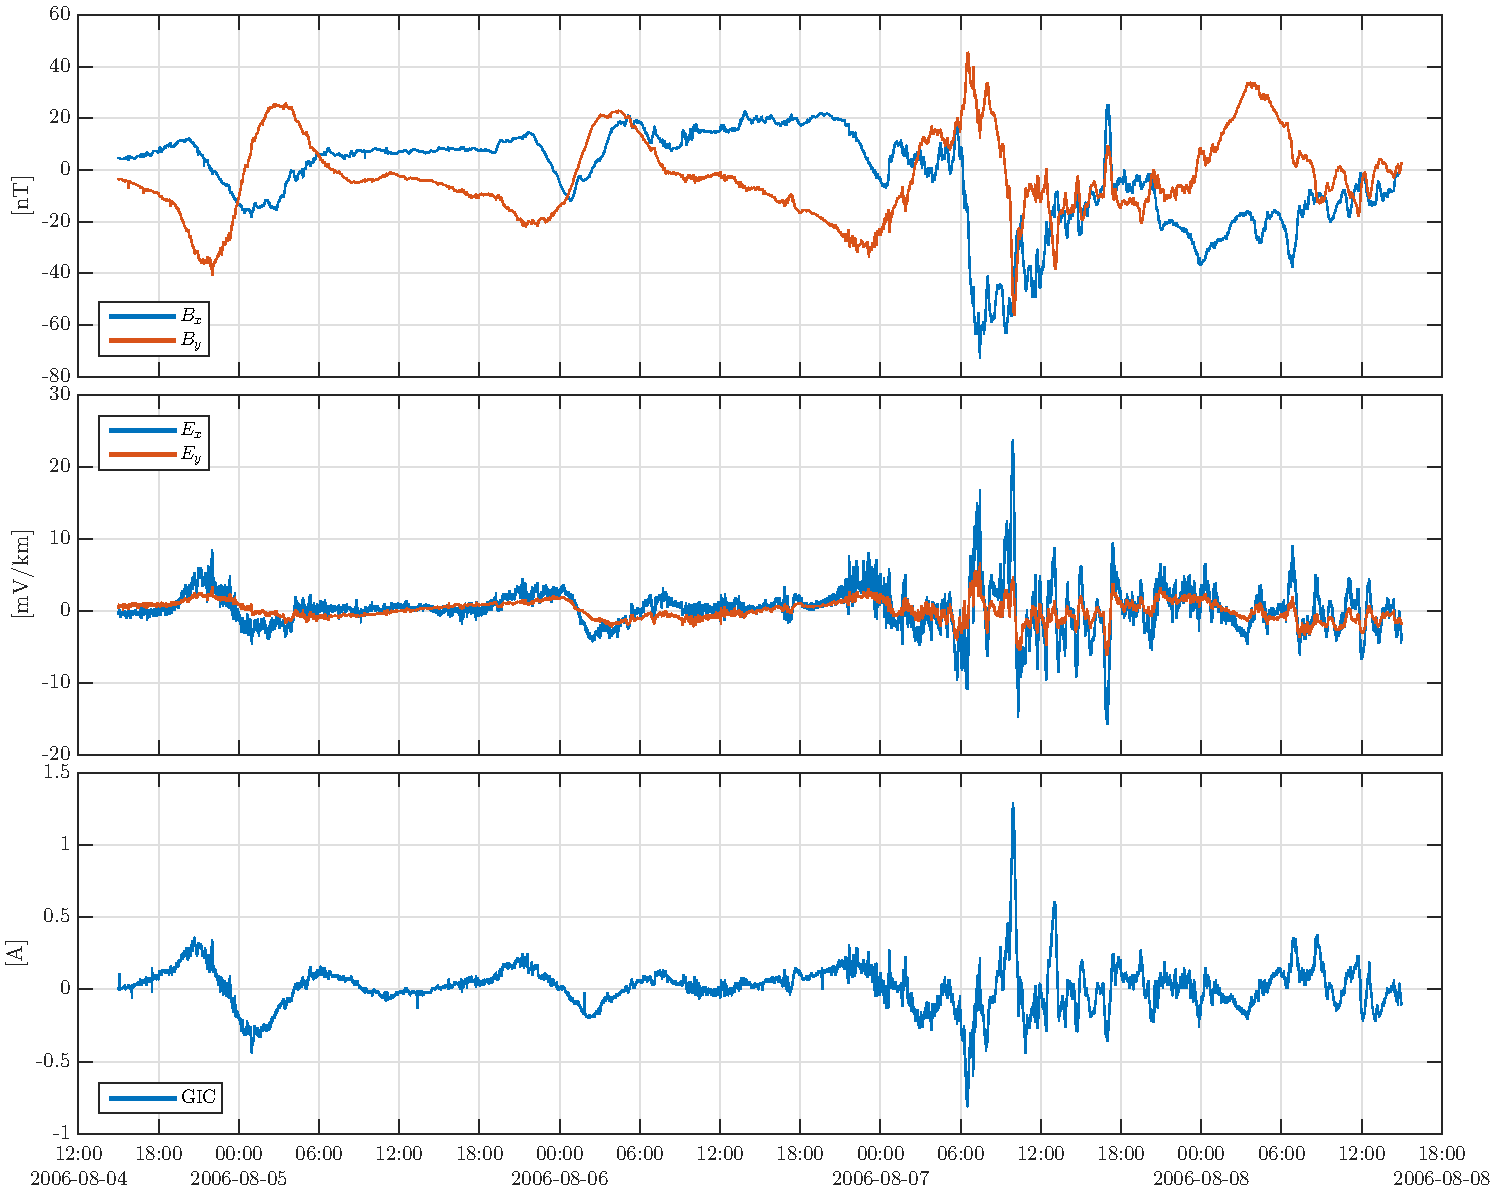
\includegraphics[width=\textwidth]{figures/plot_raw_All_20060805.pdf}
%DIFDELCMD < %%%
\DIFdelendFL \DIFaddbeginFL 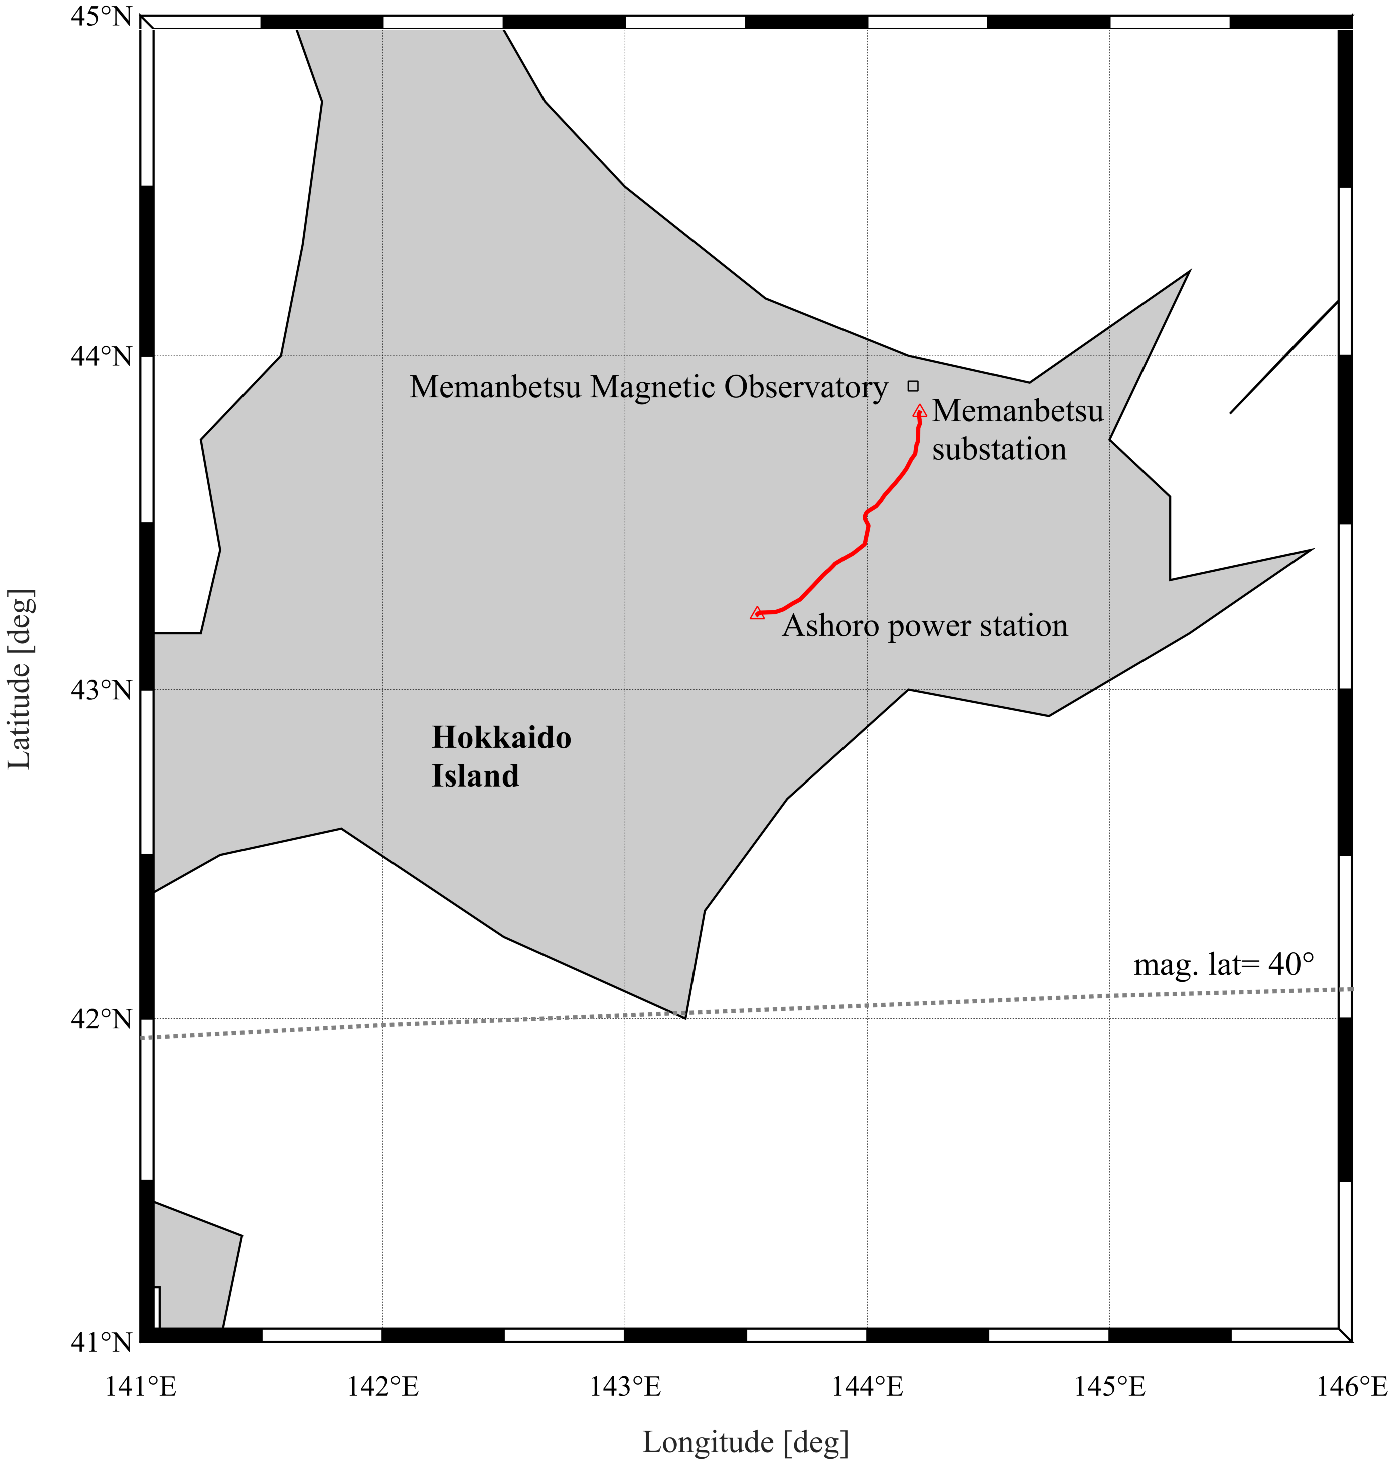
\includegraphics[width=\textwidth]{figures/map.pdf}
  \DIFaddendFL \caption{\DIFdelbeginFL \DIFdelFL{(Top) Geomagnetic field measured }\DIFdelendFL \DIFaddbeginFL \DIFaddFL{Locations of measurement sites for GIC, }\DIFaddendFL at the Memanbetsu \DIFdelbeginFL \DIFdelFL{Magnetic Observatory (MMB). (Middle) Geoelectric }\DIFdelendFL \DIFaddbeginFL \DIFaddFL{substation, and the geoelectric and geomagnetic }\DIFaddendFL field \DIFdelbeginFL \DIFdelFL{measured }\DIFdelendFL \DIFaddbeginFL \DIFaddFL{measurement site }\DIFaddendFL at \DIFdelbeginFL \DIFdelFL{the Memanbetsu }\DIFdelendFL \DIFaddbeginFL \DIFaddFL{Memambetsu }\DIFaddendFL Magnetic Observatory\DIFdelbeginFL \DIFdelFL{(MMB), which is $\sim$9 km from the Memanbetsu substation}\DIFdelendFL . \DIFdelbeginFL \DIFdelFL{(Bottom) GIC measurements measured in a grounded neutral point of a Y-connected three-phase transformer connected }\DIFdelendFL \DIFaddbeginFL \DIFaddFL{The red line corresponds }\DIFaddendFL to \DIFdelbeginFL \DIFdelFL{a 187 kV bus at }\DIFdelendFL the \DIFdelbeginFL \DIFdelFL{Memanbetsu substation }\DIFdelendFL \DIFaddbeginFL \DIFaddFL{path }\DIFaddendFL of the \DIFdelbeginFL \DIFdelFL{Hokkaido Power Co}\DIFdelendFL \DIFaddbeginFL \DIFaddFL{187 kV power line}\DIFaddendFL . The \DIFdelbeginFL \DIFdelFL{subscripts $x$ and $y$ correspond }\DIFdelendFL \DIFaddbeginFL \DIFaddFL{distance from the observatory }\DIFaddendFL to \DIFdelbeginFL \DIFdelFL{Geographic North }\DIFdelendFL \DIFaddbeginFL \DIFaddFL{the substation is $\sim$9 km }\DIFaddendFL and \DIFdelbeginFL \DIFdelFL{East, respectively.}\DIFdelendFL \DIFaddbeginFL \DIFaddFL{dotted lines are Apex geomagnetic latitudes }\citep{Richmond1995} \DIFaddFL{in 2015.}\DIFaddendFL }
  \DIFaddbeginFL \label{map}
\end{figure}

\begin{figure}[h]
  \centering
  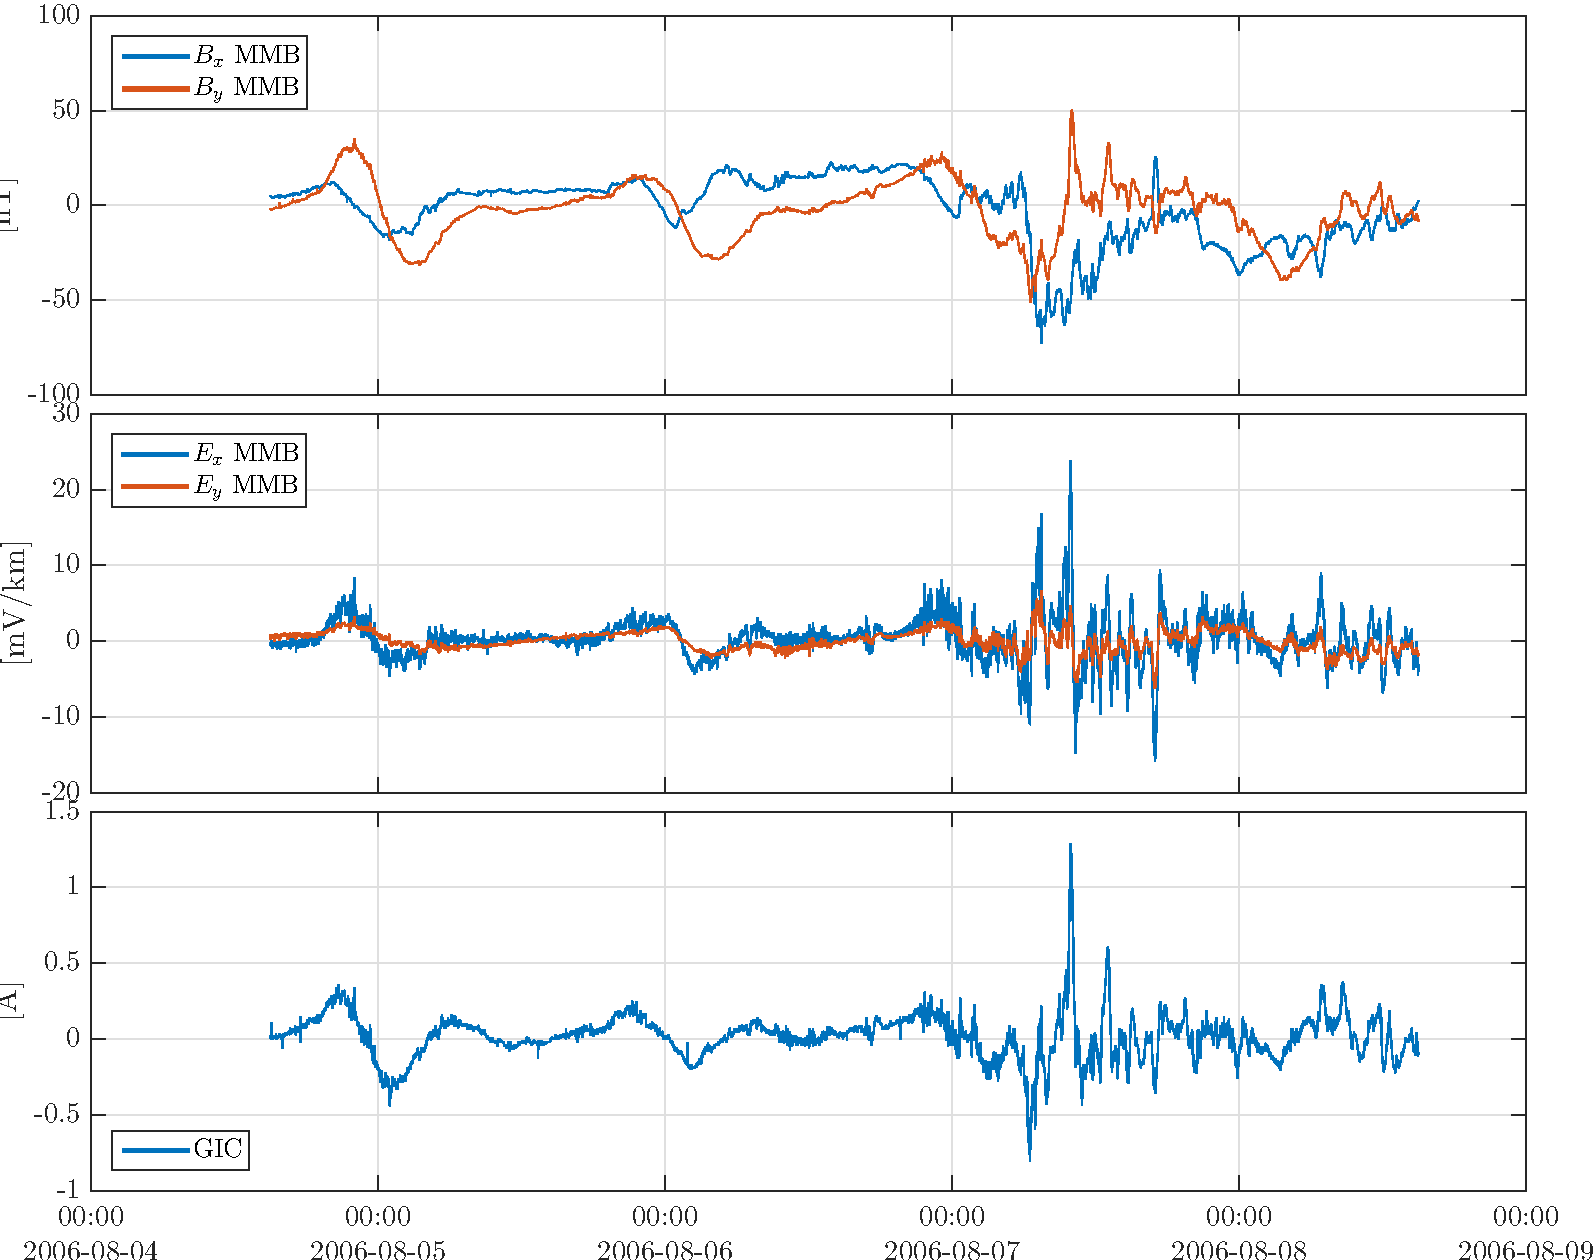
\includegraphics[width=\textwidth]{figures/plot_raw_All_20060805-v1.pdf}
  \caption{\DIFaddFL{(Top) Geomagnetic field measured at the Memanbetsu Magnetic Observatory (MMB). (Middle) Geoelectric field measured at the Memanbetsu Magnetic Observatory (MMB). (Bottom) GIC measurements at Memanbetsu substation. The subscripts $x$ and $y$ correspond to Geographic North and East, respectively, the date labels are for Universal Time, and the average have been subtracted from each time series.}}
  \DIFaddendFL \label{sample}
\end{figure}

\begin{figure}[h]
  \centering
  \DIFdelbeginFL %DIFDELCMD < 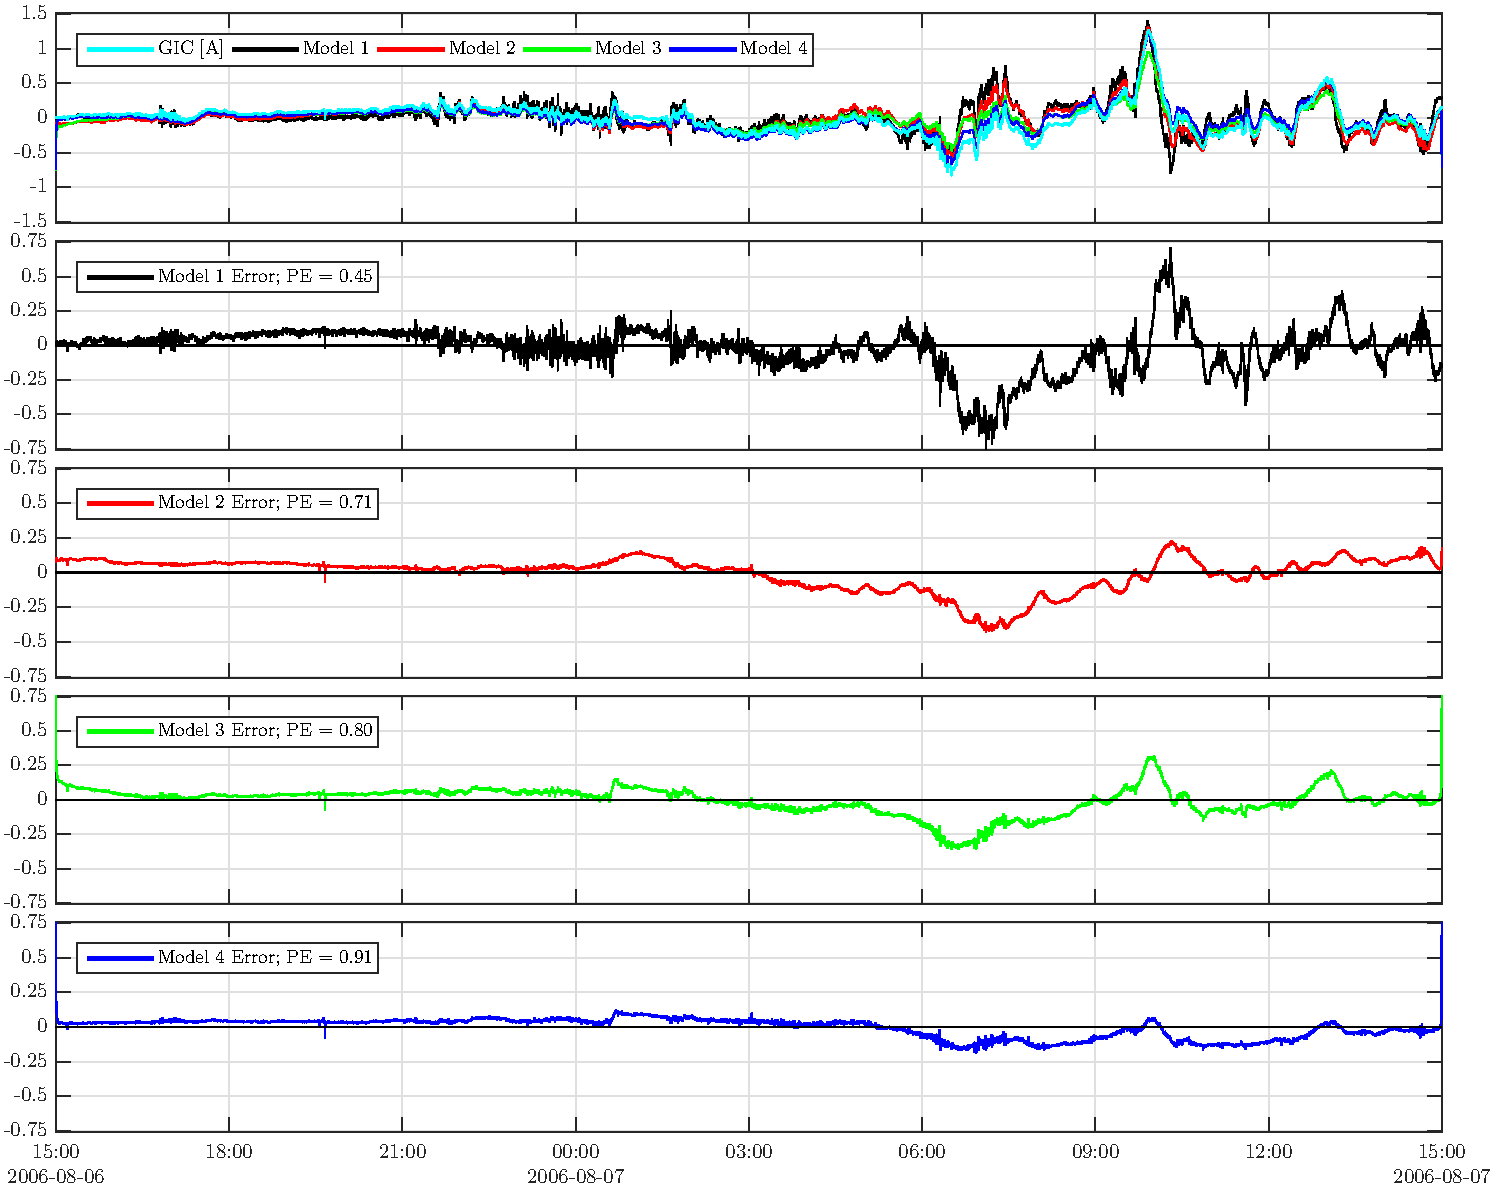
\includegraphics[width=\textwidth]{figures/plot_model_predictions-MeanModel-2006-08-06.pdf}
%DIFDELCMD < %%%
\DIFdelendFL \DIFaddbeginFL 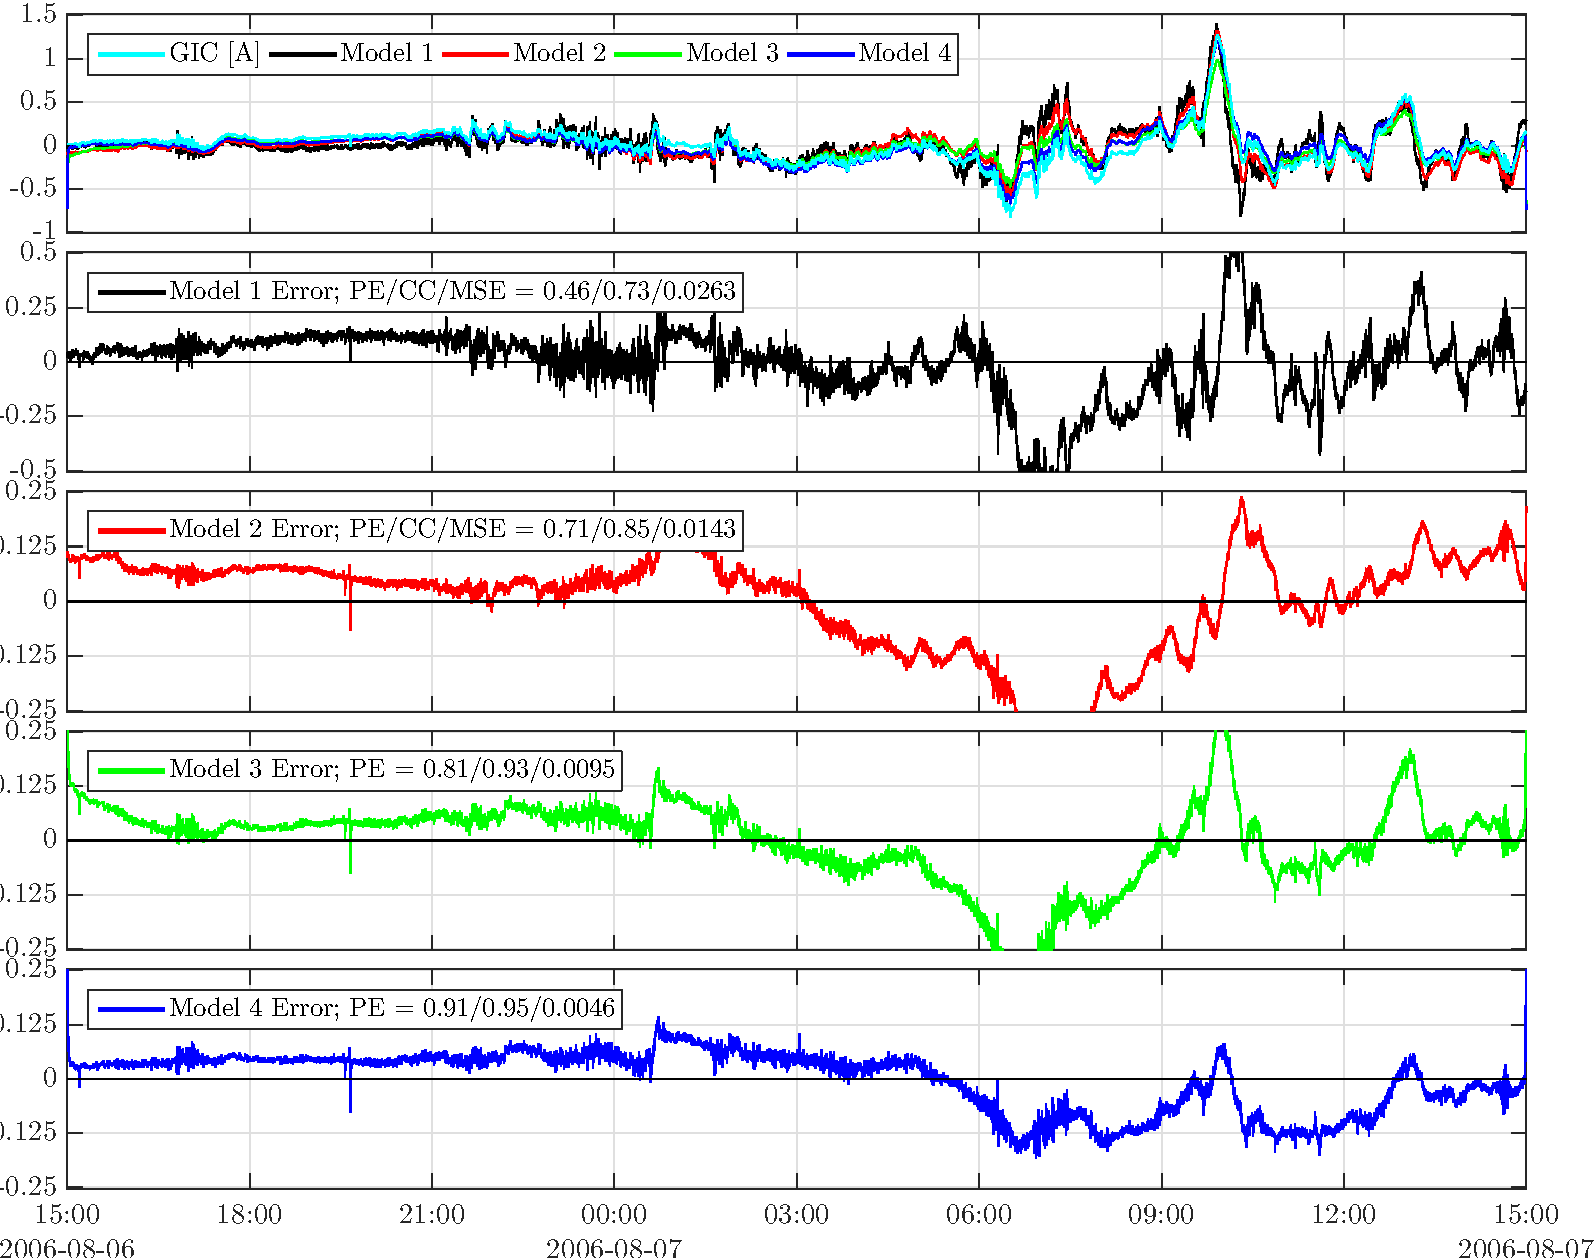
\includegraphics[width=\textwidth]{figures/plot_GIC_predictions-MeanModel-2006-08-06-v0-o0.pdf}
  \DIFaddendFL \caption{Out-of-sample model predictions (top) and predictions errors for \DIFaddbeginFL \DIFaddFL{each model in }\DIFaddendFL a \DIFaddbeginFL \DIFaddFL{selected }\DIFaddendFL 1-day interval. Note that the scales for the error time series differ from that for the top panel so that the error amplitudes are scaled up by a factor of 2.}
  \label{predictions}
\end{figure}

\begin{figure}[h]
  \centering
  \DIFdelbeginFL %DIFDELCMD < 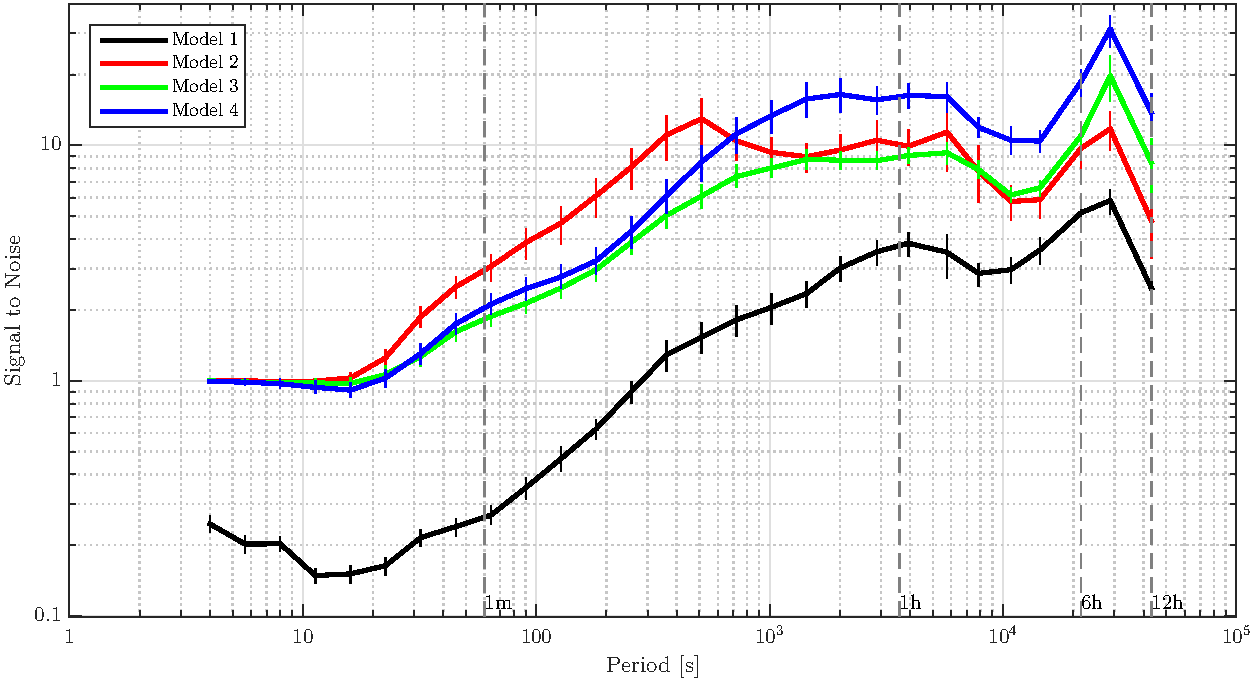
\includegraphics[width=\textwidth]{figures/plot_model_summary_SN-options-1.pdf}
%DIFDELCMD < %%%
\DIFdelendFL \DIFaddbeginFL 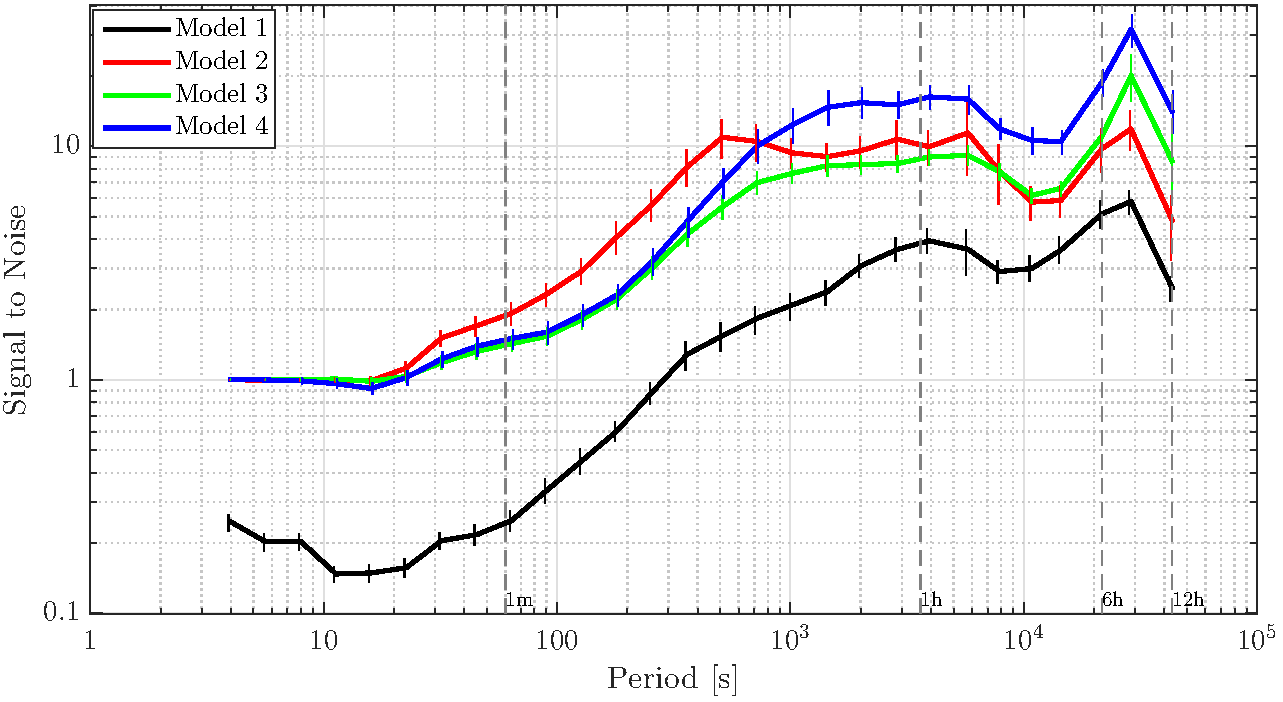
\includegraphics[width=\textwidth]{figures/plot_model_summary_SN-options-1-v0-o0.pdf}
  \DIFaddendFL \caption{Out-of-sample signal-to-noise (signal to prediction error) ratios at the evaluation frequencies for the four models.}
  \label{SN}
\end{figure}

\begin{figure}[h]
  \centering
  \DIFdelbeginFL %DIFDELCMD < 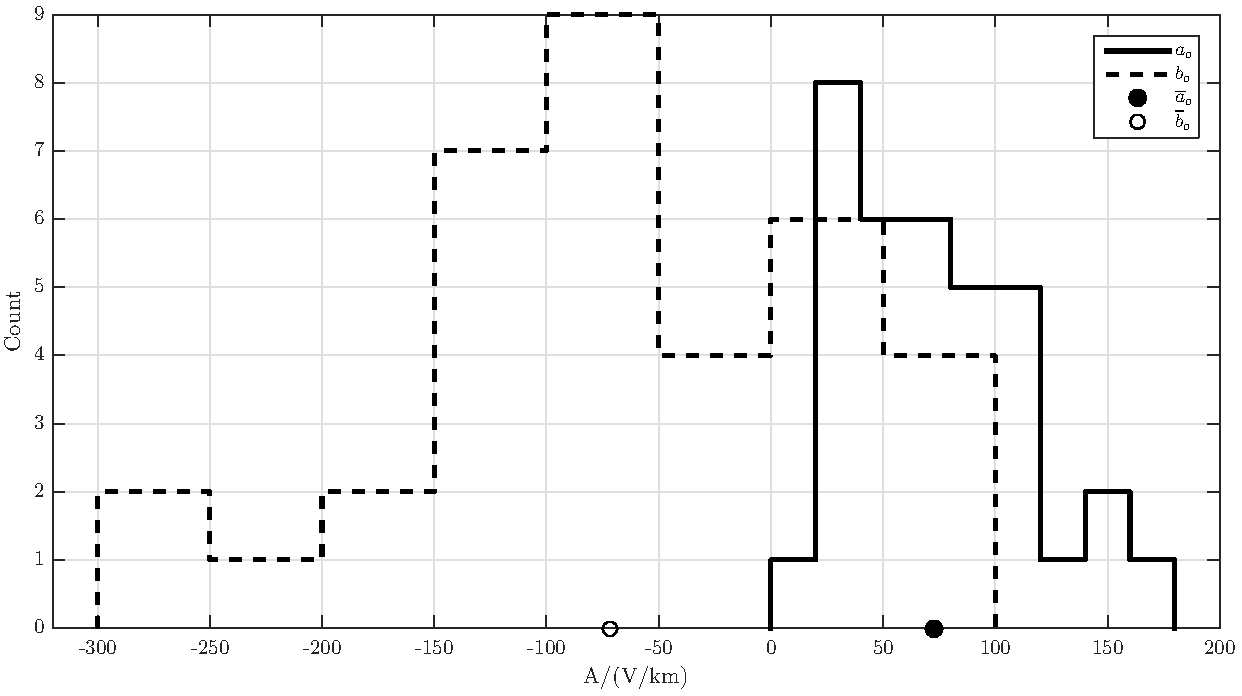
\includegraphics[width=\textwidth]{figures/plot_model_summary_aobo_histograms-options-1.pdf}
%DIFDELCMD < %%%
\DIFdelendFL \DIFaddbeginFL 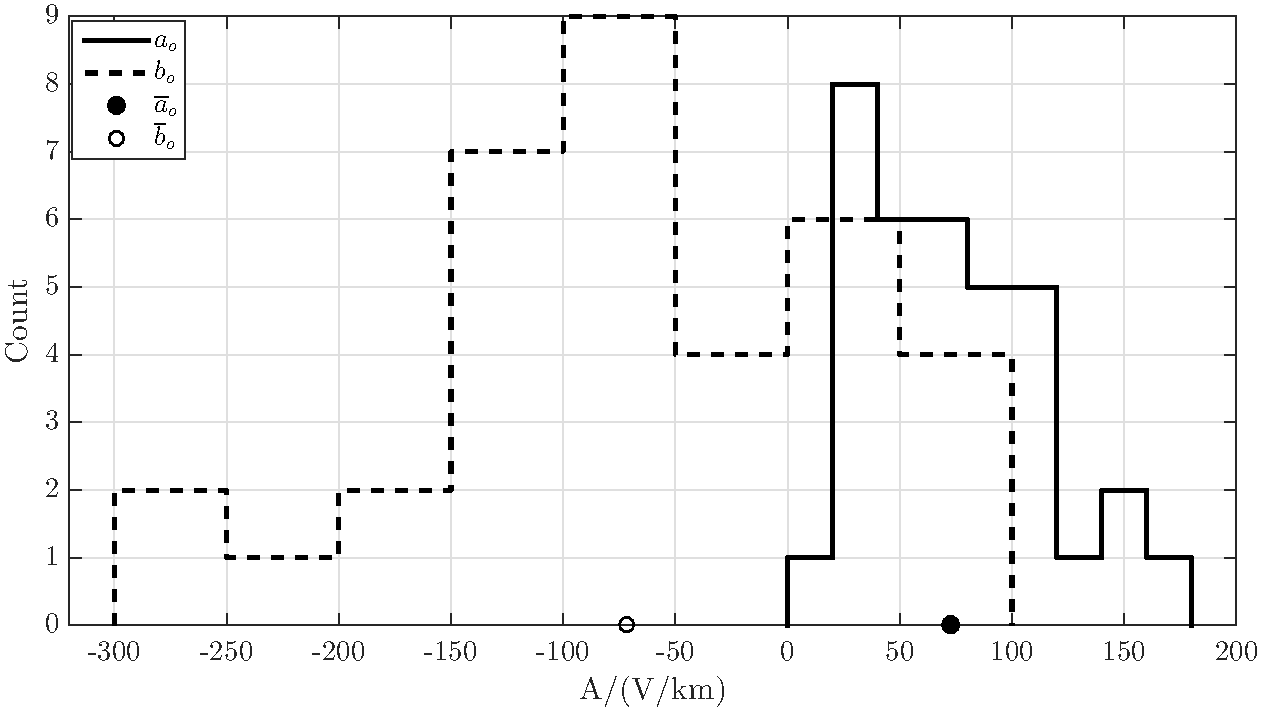
\includegraphics[width=\textwidth]{figures/plot_model_summary_aobo_histograms-options-1-v0-o0.pdf}
  \DIFaddendFL \caption{Distribution of \DIFdelbeginFL \DIFdelFL{parameters }\DIFdelendFL \DIFaddbeginFL \DIFaddFL{coefficients }\DIFaddendFL in Model\DIFaddbeginFL \DIFaddFL{~}\DIFaddendFL 1. Each set of \DIFdelbeginFL \DIFdelFL{parameters }\DIFdelendFL \DIFaddbeginFL \DIFaddFL{coefficients }\DIFaddendFL was computed 35 times using one day of 1-second cadence data. The circle \DIFdelbeginFL \DIFdelFL{/}\DIFdelendFL \DIFaddbeginFL \DIFaddFL{or }\DIFaddendFL dot on the horizontal axis indicates the average of \DIFdelbeginFL \DIFdelFL{each }\DIFdelendFL \DIFaddbeginFL \DIFaddFL{a }\DIFaddendFL histogram: $a_o$ = 73 A/(V/km) and $b_o$ = -72 A/(V/km).}
  \label{histogram}
\end{figure}

\begin{figure}[h]
  \centering
  \DIFdelbeginFL %DIFDELCMD < 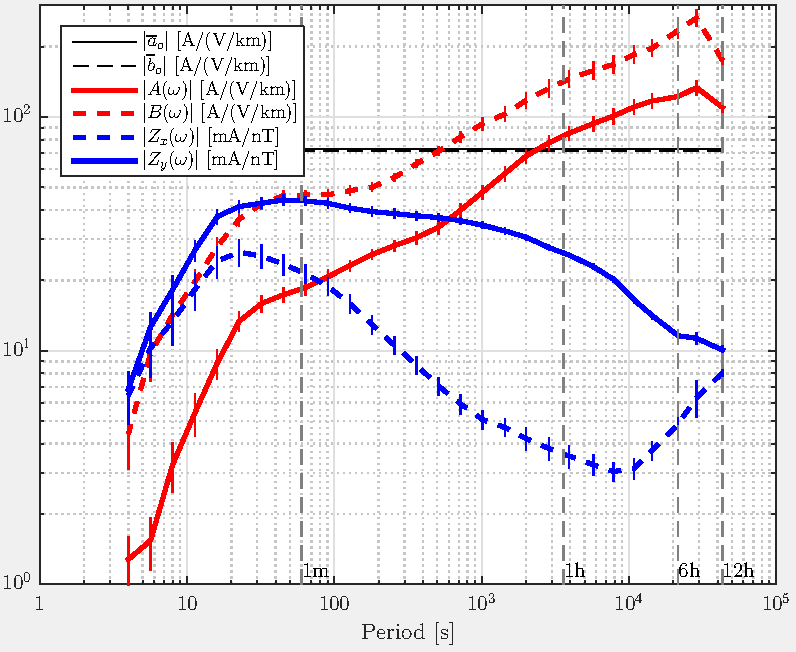
\includegraphics[width=\textwidth]{figures/plot_model_summary_Z-options-1.pdf}
%DIFDELCMD < %%%
\DIFdelendFL \DIFaddbeginFL 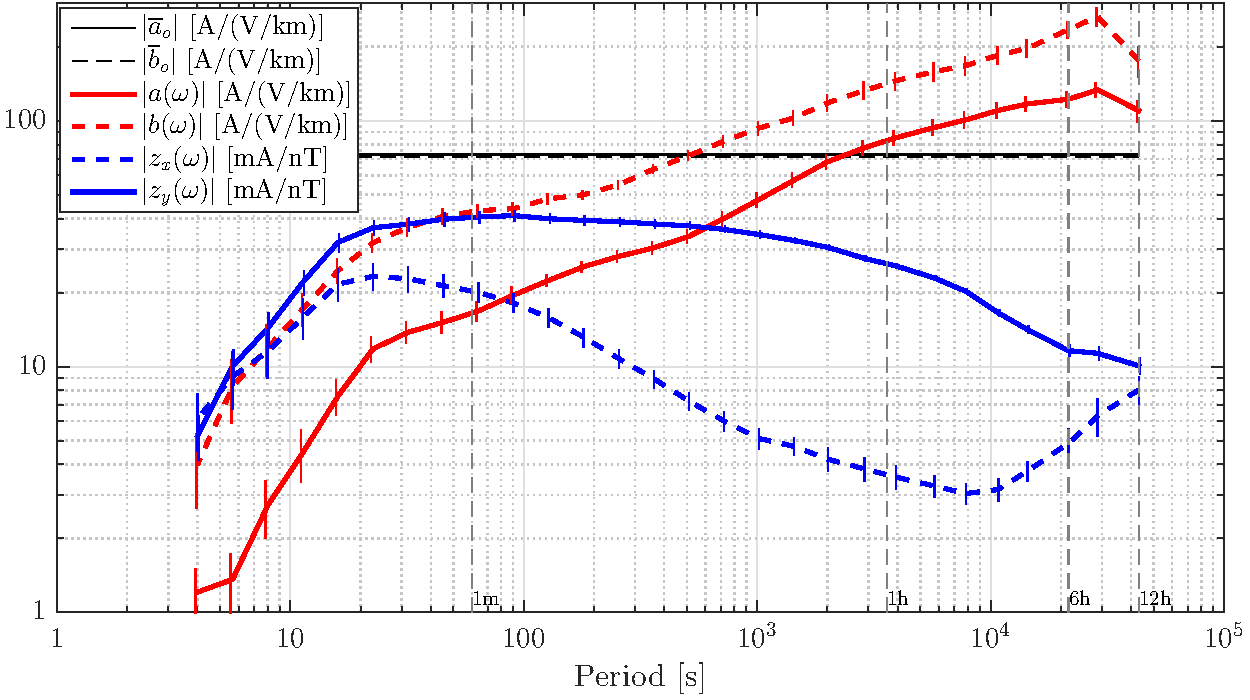
\includegraphics[width=\textwidth]{figures/plot_model_summary_Z-options-1-v0-o0.pdf}
  \DIFaddendFL \caption{Frequency domain transfer functions for the \DIFdelbeginFL \DIFdelFL{parameters }\DIFdelendFL \DIFaddbeginFL \DIFaddFL{coefficients }\DIFaddendFL in Models 1, 2, and 4. The frequency domain transfer functions for $a_o$ and $b_o$ in Model~1 are constant and equal to $a_o$ and $b_o$.}
  \label{Z}
  %\end{figure}

  \vspace{4em}

  %\begin{figure}[h]
  \centering
  \DIFdelbeginFL %DIFDELCMD < 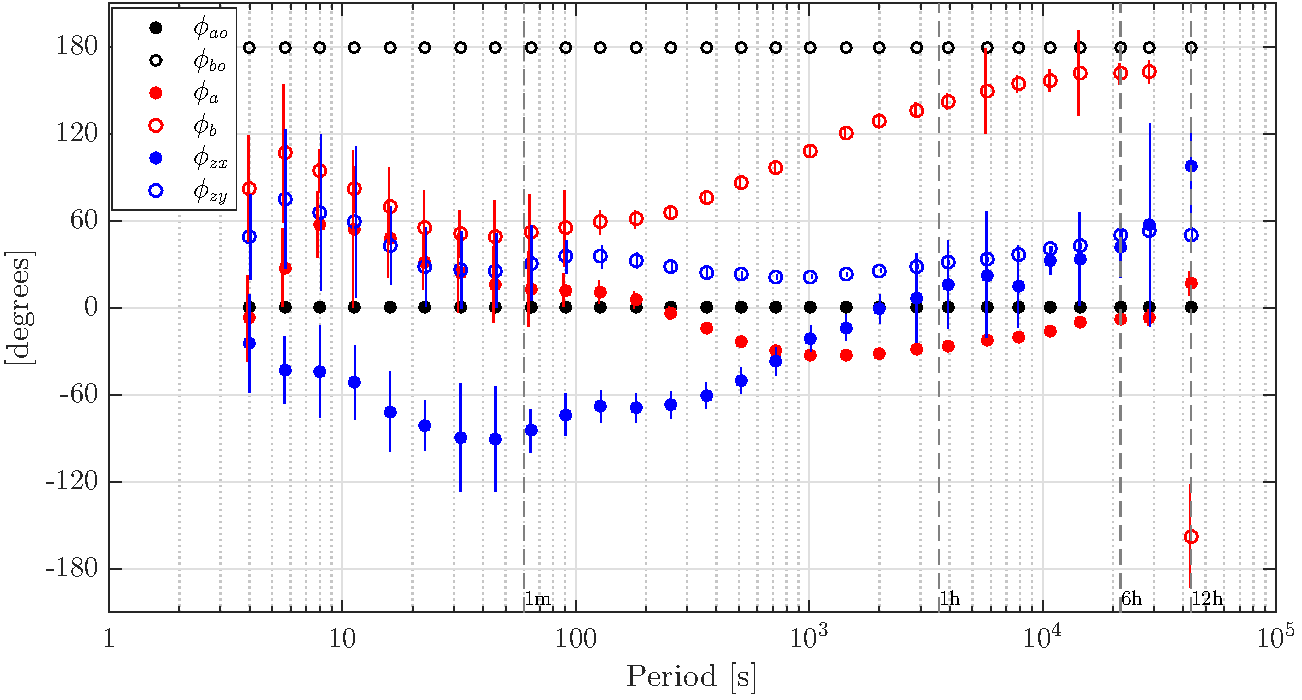
\includegraphics[width=\textwidth]{figures/plot_model_summary_Phi-options-1.pdf}
%DIFDELCMD < %%%
\DIFdelendFL \DIFaddbeginFL 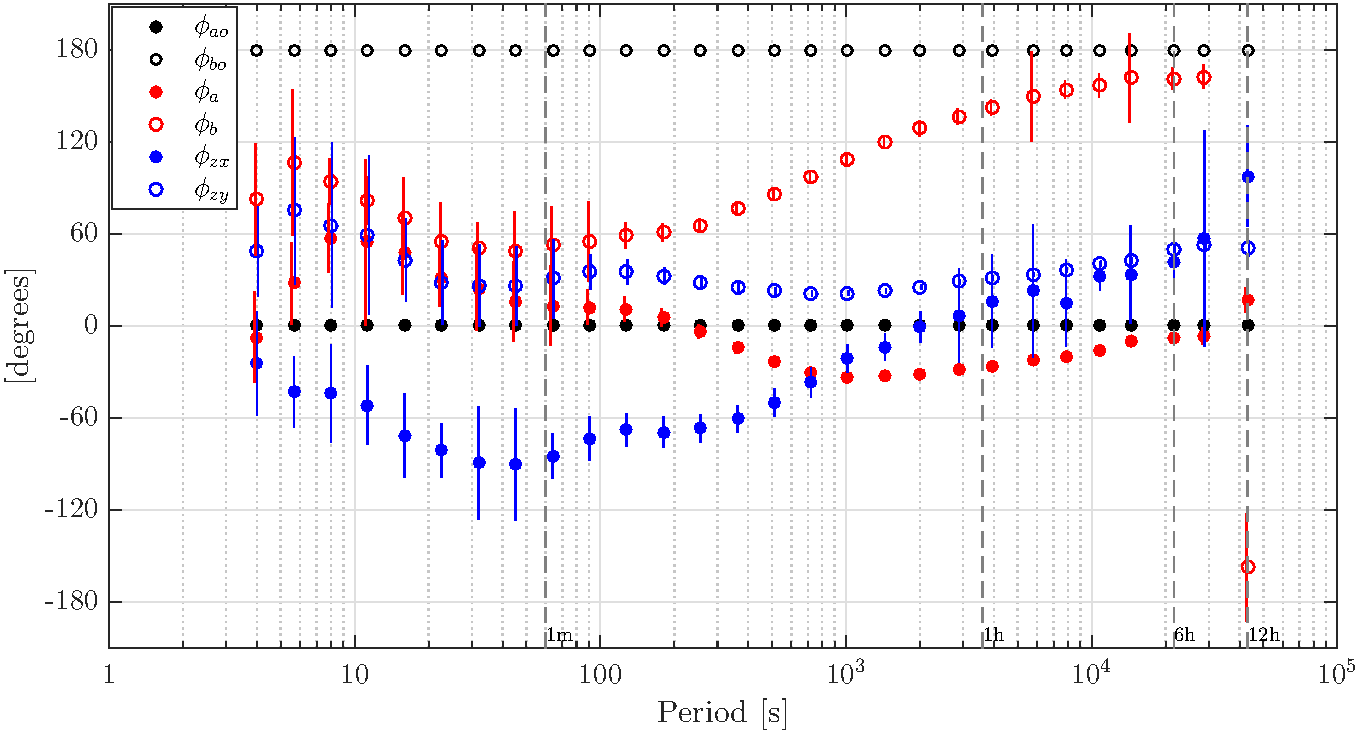
\includegraphics[width=\textwidth]{figures/plot_model_summary_Phi-options-1-v1-o0.pdf}
  \DIFaddendFL \caption{Frequency domain phase values for the \DIFdelbeginFL \DIFdelFL{parameters }\DIFdelendFL \DIFaddbeginFL \DIFaddFL{coefficients }\DIFaddendFL in Models 1, 2, and 4. The phase for $a_o$ and $b_o$ are constant and either 0\DIFdelbeginFL \DIFdelFL{$^o$ }\DIFdelendFL \DIFaddbeginFL \DIFaddFL{$^{\circ}$ }\DIFaddendFL or 180\DIFdelbeginFL \DIFdelFL{$^o$ }\DIFdelendFL \DIFaddbeginFL \DIFaddFL{$^{\circ}$ }\DIFaddendFL depending on the sign of their value, with positive values having a phase of 0\DIFdelbeginFL \DIFdelFL{$^o$}\DIFdelendFL \DIFaddbeginFL \DIFaddFL{$^{\circ}$}\DIFaddendFL .}
  \label{Phi}
\end{figure}


\begin{figure}[h]
  \centering
  \DIFdelbeginFL %DIFDELCMD < 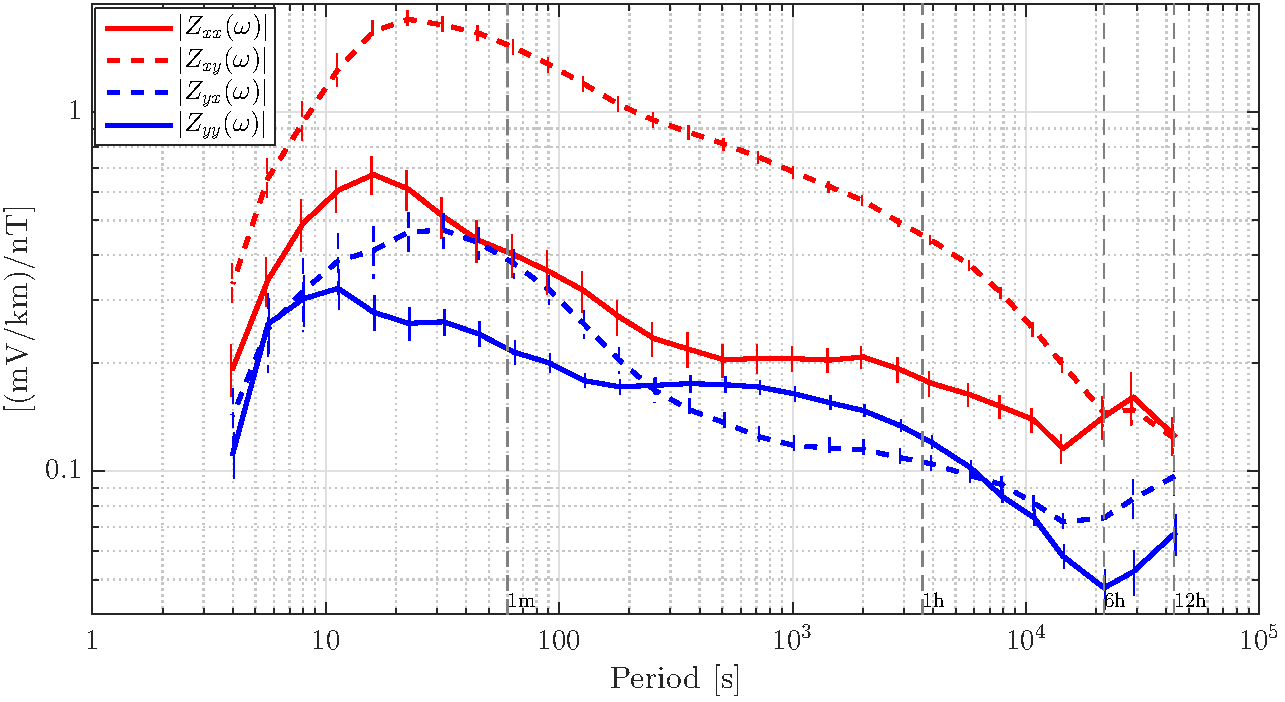
\includegraphics[width=\textwidth]{figures/plot_model_summary_Z_MT-options-1.pdf}
%DIFDELCMD < %%%
\DIFdelendFL \DIFaddbeginFL 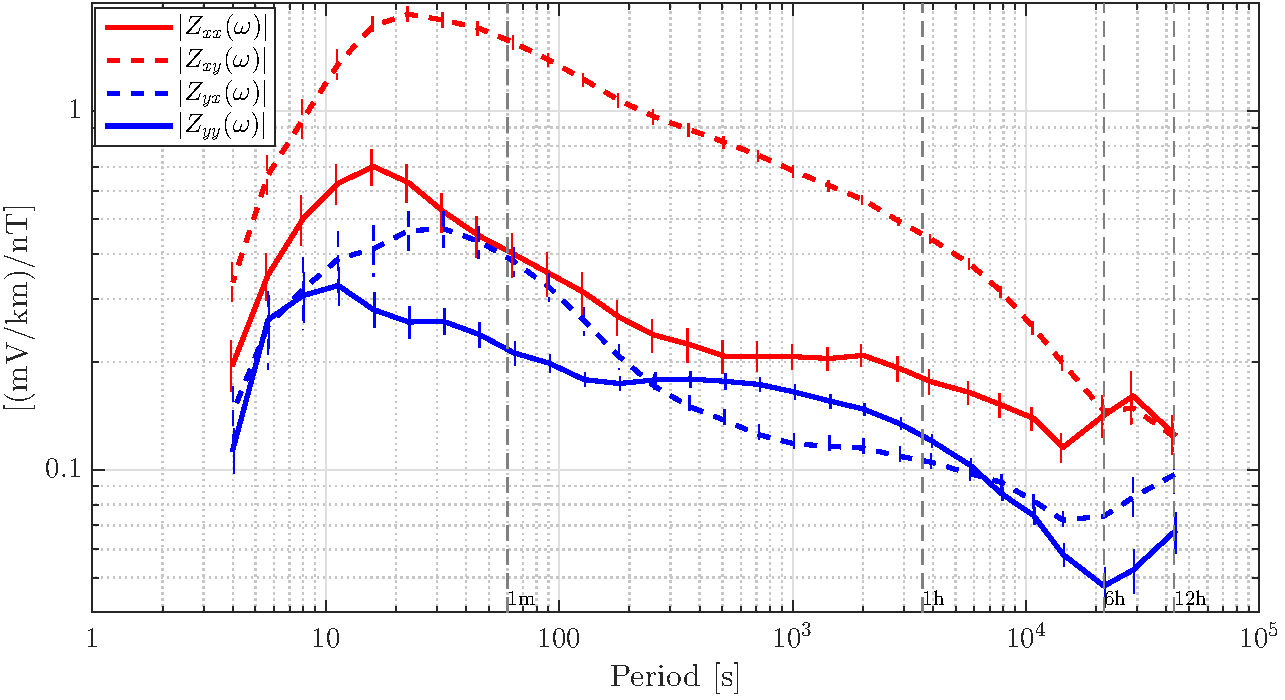
\includegraphics[width=\textwidth]{figures/plot_model_summary_Z_MT-options-1-v0-o0.pdf}
  \DIFaddendFL \caption{Frequency domain transfer functions for the \DIFdelbeginFL \DIFdelFL{parameters }\DIFdelendFL \DIFaddbeginFL \DIFaddFL{$\mathbf{Z}$ coefficients used }\DIFaddendFL in Model~3.}
  \label{Z_MT}
  %\end{figure}

  \vspace{4em}

  %\begin{figure}[h]
  \centering
  \DIFdelbeginFL %DIFDELCMD < 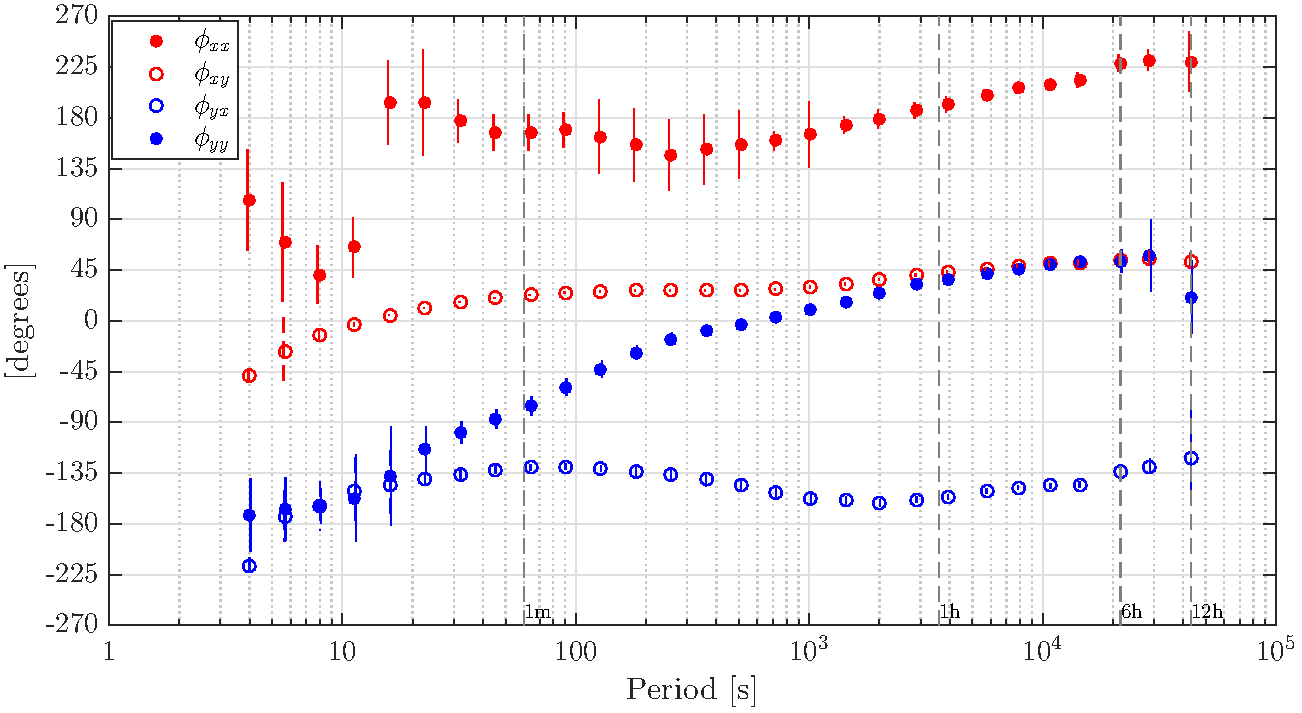
\includegraphics[width=\textwidth]{figures/plot_model_summary_Phi_MT-options-1.pdf}
%DIFDELCMD < %%%
\DIFdelendFL \DIFaddbeginFL 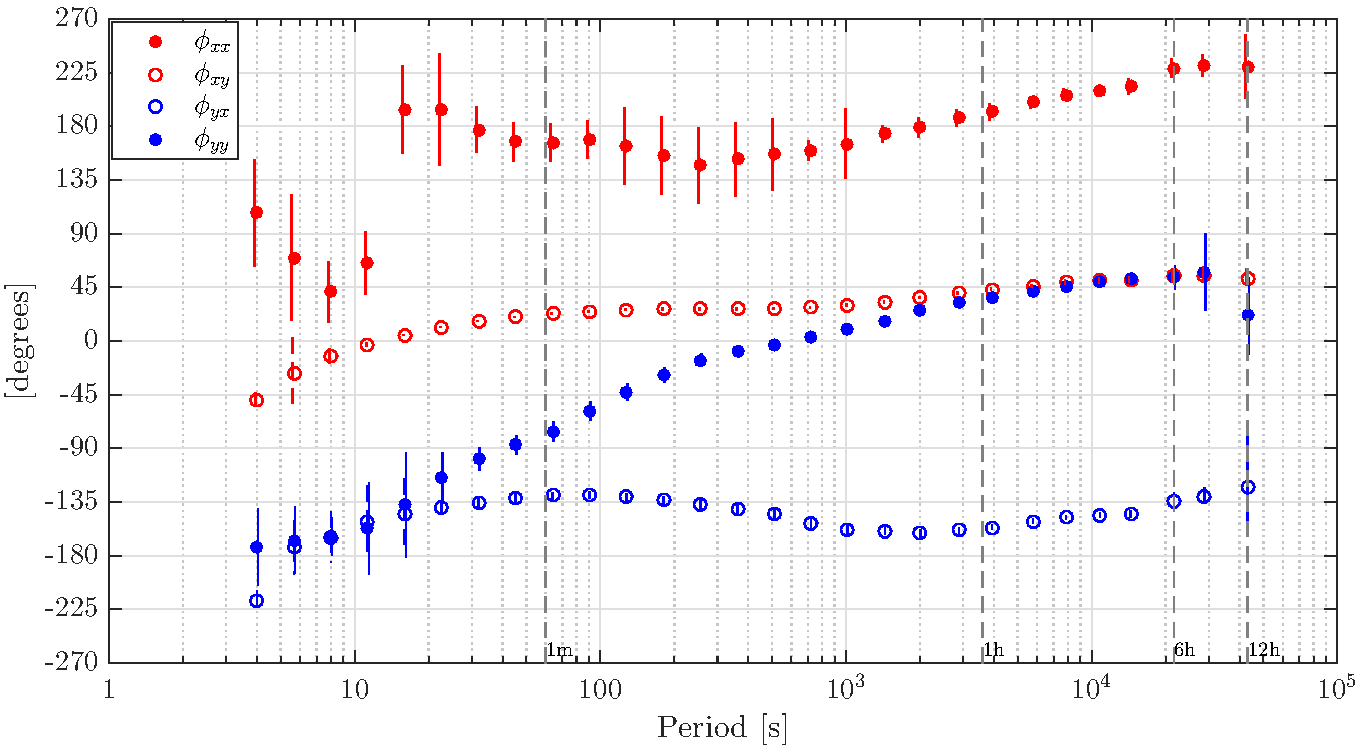
\includegraphics[width=\textwidth]{figures/plot_model_summary_Phi_MT-options-1-v1-o0.pdf}
  \DIFaddendFL \caption{Frequency domain phase values for the \DIFdelbeginFL \DIFdelFL{parameters }\DIFdelendFL \DIFaddbeginFL \DIFaddFL{$\mathbf{Z}$ coefficients used }\DIFaddendFL in Model~3.}
  \label{Phi_MT}
\end{figure}
\DIFaddbegin 

\clearpage

\section{\DIFadd{Appendix}}

\setcounter{table}{0}
\renewcommand{\thetable}{A\arabic{table}}

\begin{table}[h]
  \caption{\DIFaddFL{Date intervals used for analysis}}
  \centering
  \begin{tabular}{l l}
    \hline
    \DIFaddFL{Start Date }& \DIFaddFL{End Date}\\
    \hline
    \DIFaddFL{2006-04-03 }& \DIFaddFL{2006-04-10}\\
    \DIFaddFL{2006-07-25 }& \DIFaddFL{2006-07-29}\\
    \DIFaddFL{2006-08-05 }& \DIFaddFL{2006-08-08}\\
    \DIFaddFL{2006-08-19 }& \DIFaddFL{2006-08-21}\\
    \DIFaddFL{2006-11-07 }& \DIFaddFL{2006-11-12}\\
    \DIFaddFL{2006-11-28 }& \DIFaddFL{2006-11-29}\\
    \DIFaddFL{2006-12-01 }& \DIFaddFL{2006-12-14}\\
    \DIFaddFL{2006-12-15 }& \DIFaddFL{2006-12-15}\\
    \DIFaddFL{2007-11-18 }& \DIFaddFL{2007-11-20}\\
    \DIFaddFL{2007-11-22 }& \DIFaddFL{2007-11-22}\\
    \hline
  \end{tabular}
  \label{intervals}
\end{table}

\begin{table}
  \caption{\DIFaddFL{Periods associated with evaluation frequency bands used for regression and smoothing spectra. \# is the evaluation frequency number, $N$ is the number of DFT points in the band, and $T_e\equv 1/f_e$. The band range is from $T_l$ through $T_h$.}}
  \centering
  \begin{tabular}{l l l l l}
    \hline \\
    \DIFaddFL{\# }& \DIFaddFL{$N$ }& \DIFaddFL{$T_e$ }[\DIFaddFL{s}] & \DIFaddFL{$T_l$ }[\DIFaddFL{s}] & \DIFaddFL{$T_h$ }[\DIFaddFL{s}] \\
    \hline \\
    \DIFaddFL{1 }& \DIFaddFL{2 }& \DIFaddFL{43200 }& \DIFaddFL{28800 }& \DIFaddFL{86400 }\\
    \DIFaddFL{2 }& \DIFaddFL{2 }& \DIFaddFL{28800 }& \DIFaddFL{21600 }& \DIFaddFL{43200 }\\
    \DIFaddFL{3 }& \DIFaddFL{3 }& \DIFaddFL{21600 }& \DIFaddFL{14400 }& \DIFaddFL{43200 }\\
    \DIFaddFL{4 }& \DIFaddFL{4 }& \DIFaddFL{14400 }& \DIFaddFL{9600 }& \DIFaddFL{28800 }\\
    \DIFaddFL{5 }& \DIFaddFL{5 }& \DIFaddFL{10800 }& \DIFaddFL{7200 }& \DIFaddFL{21600 }\\
    \DIFaddFL{6 }& \DIFaddFL{6 }& \DIFaddFL{7854.5 }& \DIFaddFL{5400 }& \DIFaddFL{14400 }\\
    \DIFaddFL{7 }& \DIFaddFL{8 }& \DIFaddFL{5760 }& \DIFaddFL{3927.3 }& \DIFaddFL{10800 }\\
    \DIFaddFL{8 }& \DIFaddFL{12 }& \DIFaddFL{3927.3 }& \DIFaddFL{2618.2 }& \DIFaddFL{7854.5 }\\
    \DIFaddFL{9 }& \DIFaddFL{16 }& \DIFaddFL{2880 }& \DIFaddFL{1920 }& \DIFaddFL{5760 }\\
    \DIFaddFL{10 }& \DIFaddFL{22 }& \DIFaddFL{2009.3 }& \DIFaddFL{1350 }& \DIFaddFL{3927.3 }\\
    \DIFaddFL{11 }& \DIFaddFL{31 }& \DIFaddFL{1440 }& \DIFaddFL{960 }& \DIFaddFL{2880 }\\
    \DIFaddFL{12 }& \DIFaddFL{43 }& \DIFaddFL{1016.5 }& \DIFaddFL{680.3 }& \DIFaddFL{2009.3 }\\
    \DIFaddFL{13 }& \DIFaddFL{61 }& \DIFaddFL{720 }& \DIFaddFL{480 }& \DIFaddFL{1440 }\\
    \DIFaddFL{14 }& \DIFaddFL{85 }& \DIFaddFL{511.2 }& \DIFaddFL{341.5 }& \DIFaddFL{1016.5 }\\
    \DIFaddFL{15 }& \DIFaddFL{120 }& \DIFaddFL{361.5 }& \DIFaddFL{241.3 }& \DIFaddFL{720 }\\
    \DIFaddFL{16 }& \DIFaddFL{170 }& \DIFaddFL{255.6 }& \DIFaddFL{170.4 }& \DIFaddFL{511.2 }\\
    \DIFaddFL{17 }& \DIFaddFL{240 }& \DIFaddFL{180.8 }& \DIFaddFL{120.5 }& \DIFaddFL{361.5 }\\
    \DIFaddFL{18 }& \DIFaddFL{338 }& \DIFaddFL{128 }& \DIFaddFL{85.4 }& \DIFaddFL{255.6 }\\
    \DIFaddFL{19 }& \DIFaddFL{478 }& \DIFaddFL{90.5 }& \DIFaddFL{60.3 }& \DIFaddFL{180.8 }\\
    \DIFaddFL{20 }& \DIFaddFL{676 }& \DIFaddFL{64 }& \DIFaddFL{42.7 }& \DIFaddFL{128 }\\
    \DIFaddFL{21 }& \DIFaddFL{956 }& \DIFaddFL{45.2 }& \DIFaddFL{30.2 }& \DIFaddFL{90.5 }\\
    \DIFaddFL{22 }& \DIFaddFL{1351 }& \DIFaddFL{32 }& \DIFaddFL{21.3 }& \DIFaddFL{64 }\\
    \DIFaddFL{23 }& \DIFaddFL{1910 }& \DIFaddFL{22.6 }& \DIFaddFL{15.1 }& \DIFaddFL{45.2 }\\
    \DIFaddFL{24 }& \DIFaddFL{2701 }& \DIFaddFL{16 }& \DIFaddFL{10.7 }& \DIFaddFL{32 }\\
    \DIFaddFL{25 }& \DIFaddFL{3819 }& \DIFaddFL{11.3 }& \DIFaddFL{7.5 }& \DIFaddFL{22.6 }\\
    \DIFaddFL{26 }& \DIFaddFL{5401 }& \DIFaddFL{8 }& \DIFaddFL{5.3 }& \DIFaddFL{16 }\\
    \DIFaddFL{27 }& \DIFaddFL{7638 }& \DIFaddFL{5.7 }& \DIFaddFL{3.8 }& \DIFaddFL{11.3 }\\
    \DIFaddFL{28 }& \DIFaddFL{10801 }& \DIFaddFL{4 }& \DIFaddFL{2.7 }& \DIFaddFL{8 }\\
    \hline \\
  \end{tabular}
  \label{evaluationperiods}
\end{table}
\DIFaddend 

\clearpage

\bibliography{paper.bib}

\end{document}
